%
% Vienna University of Technology - Faculty of Informatics
% TUINF thesis - LaTeX template
%
% For questions and comments send an email to
% Thomas Auzinger <thomas.auzinger@cg.tuwien.ac.at>
% Thomas Krennwallner <tkren@kr.tuwien.ac.at>
%
% ---------------------------------------------------------
%
% TU Wien - Fakultät für Informatik
% TUINF Arbeit - Template für LaTeX
%
% Für Fragen oder Kommentare schicken Sie eine Email an
% Thomas Auzinger <thomas.auzinger@cg.tuwien.ac.at>
% Thomas Krennwallner <tkren@kr.tuwien.ac.at>
%

\documentclass[a4paper,11pt]{memoir}
\chapterstyle{veelo}

\usepackage{TUINFTHESIS}

\usepackage{geometry}[2010/02/15] % page geometry (\newgeometry command needs a recent version)
\usepackage{url}      % URL functionality
\usepackage{hyperref} % hyperlinks in PDF files
\usepackage{graphicx} % images
\usepackage{verbatim} % code environments
\usepackage[lined,linesnumbered,algochapter]{algorithm2e} % algorithm environments

\usepackage{pgf}  % graphics
\usepackage{tikz}	% graphics
\usetikzlibrary{arrows,automata}

\usepackage{ngerman}           % support for German
\usepackage[ngerman]{babel}    % support for German
\usepackage{bibgerm,cite}      % German notations
\usepackage[ngerman]{varioref} % German references
% to use the german charset include cp850 for MS-DOS, ansinew for Windows and latin1 for Linux.
% \usepackage[latin1]{inputenc}

% enable hyphenation of urls at every location (to avoid bad boxes)
\renewcommand{\UrlBreaks}{\do\/\do\a\do\b\do\c\do\d\do\e\do\f\do\g\do\h\do\i\do\j\do\k\do\l\do\m\do\n\do\o\do\p\do\q\do\r\do\s\do\t\do\u\do\v\do\w\do\x\do\y\do\z\do\A\do\B\do\C\do\D\do\E\do\F\do\G\do\H\do\I\do\J\do\K\do\L\do\M\do\N\do\O\do\P\do\Q\do\R\do\S\do\T\do\U\do\V\do\W\do\X\do\Y\do\Z}

% all the following \thesis... definitions are mandatory unless declared optional
\thesistitle{Visualization of Composite Objects Through Techniques of Exploded Views and Ghosting}
\thesissubtitle{}% optional
\thesisdate{12.12.2013}
\thesislocation{Wien}

\thesistype{bachelor} % master or bachelor
\thesiscurriculum{Medieninformatik und Visual Computing}{Media Informatics and Visual Computing} % German and English

\thesisauthorname{Hartwig Wutscher}
\thesisauthorgender{male} % female or male
\thesisauthoraddress{Nesselgasse 4/22, 1170 Wien}
\thesismatrikelno{0426961}

\thesisadvisorname{o.Univ.-Prof. Dipl.-Ing. Mag. Dr. Monika Musterprofessorin}
\thesisadvisorgender{male} % female or male
\thesisassistantonename{Ma. Sc. Peter Mindek}

\begin{document}

\captionnamefont{\bfseries}

% define page numbering styles
\makepagestyle{numberCorner}
\makeevenfoot{numberCorner}{\thepage}{}{}
\makeoddfoot{numberCorner}{}{}{\thepage}

%%%%%%%%%%%%%%%%%%%%%%%%%%%%%%%%%%%%%%%%%
%%%   FRONTMATTER    %%%%%%%%%%%%%%%%%%%%
%%%%%%%%%%%%%%%%%%%%%%%%%%%%%%%%%%%%%%%%%
\frontmatter
\pagenumbering{roman}

%%%%%%%%%%%%%%%%%%%%%%%%%%%%%%%%%%%%%%%%%
%%%   TITLE PAGES    %%%%%%%%%%%%%%%%%%%%
%%%%%%%%%%%%%%%%%%%%%%%%%%%%%%%%%%%%%%%%%
%
% Vienna University of Technology - Faculty of Informatics
% TUINF thesis - Title page German
%
% For questions and comments send an email to
% Thomas Auzinger <thomas.auzinger@cg.tuwien.ac.at>
% Thomas Krennwallner <tkren@kr.tuwien.ac.at>
%
% ---------------------------------------------------------
%
% TU Wien - Fakult�t f�r Informatik
% TUINF Arbeit - Titelseite deutsch
%
% F�r Fragen oder Kommentare schicken Sie eine Email an
% Thomas Auzinger <thomas.auzinger@cg.tuwien.ac.at>
% Thomas Krennwallner <tkren@kr.tuwien.ac.at>
%

\selectlanguage{ngerman}

% setup page dimensions for the titlepage
\newgeometry{left=2.4cm,right=2.4cm,bottom=2.5cm,top=2cm}

% force baselineskip and parindent
\newlength{\tmpbaselineskip}
\setlength{\tmpbaselineskip}{\baselineskip}
\setlength{\baselineskip}{13.6pt}
\newlength{\tmpparindent}
\setlength{\tmpparindent}{\parindent}
\setlength{\parindent}{17pt}

% title page
\thispagestyle{tuinftitlepage}

% Prevent warning messages due to tall headers
\addtolength{\headheight}{65pt}
\addtolength{\headsep}{-65pt}

%
% Kludge: for each titlepage set \pagenumbering to a different
% style. This is used to fix a problem with hyperref, because there
% are multiple "page 1" and hyperref hates that
%
\pagenumbering{Roman}

\begin{center}
{\ \vspace{3.4cm}}

\begin{minipage}[t][2.8cm][s]{\textwidth}%
\centering
\thesistitlefontHUGE\sffamily\bfseries\tuinfthesistitle\\
\bigskip
{\thesistitlefonthuge\sffamily\bfseries\tuinfthesissubtitle}
\end{minipage}

\vspace{1.3cm}

{\thesistitlefontLARGE\sffamily \tuinfthesistypename}

\vspace{6mm}

{\thesistitlefontlarge\sffamily zur Erlangung des akademischen Grades}

\vspace{6mm}

{\thesistitlefontLARGE\sffamily\bfseries \tuinfthesisdegree}

\vspace{6mm}

{\thesistitlefontlarge\sffamily im Rahmen des Studiums}

\vspace{6mm}

{\thesistitlefontLarge\sffamily\bfseries \tuinfthesiscurriculum}

\vspace{6.5mm}

{\thesistitlefontlarge\sffamily eingereicht von}

\vspace{6mm}

{\thesistitlefontLarge\sffamily\bfseries \tuinfthesisauthorname}

\vspace{1.5mm}

{\thesistitlefontlarge\sffamily Matrikelnummer \tuinfthesismatrikelno} 

\vspace{1.4cm}

\begin{minipage}[t][1.6cm][t]{\textwidth}%
	\vspace{0pt}\raggedright\thesistitlefontnormalsize\sffamily%
  an der Fakult\"{a}t f\"{u}r Informatik
	
	der Technischen Universit\"{a}t Wien
\end{minipage}

\begin{minipage}[t][4cm][t]{\textwidth}%
  \vspace{0pt}\raggedright\thesistitlefontnormalsize\sffamily%
  \begin{tabbing}%
	    \hspace{19mm} \= \hspace{66mm} \kill
	    Betreuung: \> \tuinfthesisadvisorname\\
	    Mitwirkung: \> \tuinfthesisassistantonename\\
	                \> \tuinfthesisassistanttwoname
  \end{tabbing}
\end{minipage}

\begin{minipage}[t][1.5cm][t]{\textwidth}%
  \vspace{0pt}\sffamily\thesistitlefontnormalsize
  \begin{tabbing}%
    \hspace{45mm} \= \hspace{63mm} \= \hspace{51mm} \kill
    Wien, \tuinfthesisdate \> {\raggedright\rule{51mm}{0.5pt}} \> {\raggedright\rule{51mm}{0.5pt}} \\
    \> \begin{minipage}[t][0.5cm][t]{51mm}\centering (Unterschrift \tuinfthesisverfasser)\end{minipage}
    \> \begin{minipage}[t][0.5cm][t]{51mm}\centering (Unterschrift \tuinfthesisbetreuer)\end{minipage}
    \end{tabbing}
\end{minipage}

\end{center}

% we want an empty page right after first titlepage
\pagestyle{empty}
\cleardoublepage

% we're done with the titlepages, proceed with default pagenumbering
\pagenumbering{roman}

% restore baselineskip
\setlength{\baselineskip}{\tmpbaselineskip}
\setlength{\parindent}{\tmpparindent}

% back to normal geometry
\restoregeometry % the German title page is required as first page
%
% Vienna University of Technology - Faculty of Informatics
% TUINF thesis - Title page English
%
% For questions and comments send an email to
% Thomas Auzinger <thomas.auzinger@cg.tuwien.ac.at>
% Thomas Krennwallner <tkren@kr.tuwien.ac.at>
%
% ---------------------------------------------------------
%
% TU Wien - Fakult�t f�r Informatik
% TUINF Arbeit - Titelseite englisch
%
% F�r Fragen oder Kommentare schicken Sie eine Email an
% Thomas Auzinger <thomas.auzinger@cg.tuwien.ac.at>
% Thomas Krennwallner <tkren@kr.tuwien.ac.at>
%

\selectlanguage{english}

% setup page dimensions for the titlepage
\newgeometry{left=2.4cm,right=2.4cm,bottom=2.5cm,top=2cm}

% force baselineskip and parindent
\newlength{\tmpbaselineskipen}
\setlength{\tmpbaselineskipen}{\baselineskip}
\setlength{\baselineskip}{13.6pt}
\newlength{\tmpparindenten}
\setlength{\tmpparindenten}{\parindent}
\setlength{\parindent}{17pt}

% title page
\thispagestyle{tuinftitlepage}

% Prevent warning messages due to tall headers
\addtolength{\headheight}{65pt}
\addtolength{\headsep}{-65pt}

%
% Kludge: for each titlepage set \pagenumbering to a different
% style. This is used to fix a problem with hyperref, because there
% are multiple "page 1" and hyperref hates that
%
\pagenumbering{Alph}

\begin{center}
{\ \vspace{3.4cm}}

\begin{minipage}[t][2.8cm][s]{\textwidth}%
\centering
\thesistitlefontHUGE\sffamily\bfseries\tuinfthesistitle\\
\bigskip
{\thesistitlefonthuge\sffamily\bfseries\tuinfthesissubtitle}
\end{minipage}

\vspace{1.3cm}

{\thesistitlefontLARGE\sffamily \tuinfthesistypenameen}

\vspace{6mm}

{\thesistitlefontlarge\sffamily submitted in partial fulfillment of the requirements for the degree of}

\vspace{6mm}

{\thesistitlefontLARGE\sffamily\bfseries \tuinfthesisdegree}

\vspace{6mm}

{\thesistitlefontlarge\sffamily in}

\vspace{6mm}

{\thesistitlefontLarge\sffamily\bfseries \tuinfthesiscurriculumen}

\vspace{6.5mm}

{\thesistitlefontlarge\sffamily by}

\vspace{6mm}

{\thesistitlefontLarge\sffamily\bfseries \tuinfthesisauthorname}

\vspace{1.5mm}

{\thesistitlefontlarge\sffamily Registration Number \tuinfthesismatrikelno} 

\vspace{1.4cm}

\begin{minipage}[t][1.6cm][t]{\textwidth}%
  \vspace{0pt}\raggedright\thesistitlefontnormalsize\sffamily%
  to the Faculty of Informatics 

  at the Vienna University of Technology
\end{minipage}

\begin{minipage}[t][4cm][t]{\textwidth}%
	\vspace{0pt}\raggedright\thesistitlefontnormalsize\sffamily
  \begin{tabbing}%
	    \hspace{19mm} \= \hspace{66mm} \kill
	    Advisor: \> \tuinfthesisadvisorname\\
	    Assistance: \> \tuinfthesisassistantonename\\
	                \> \tuinfthesisassistanttwoname
   \end{tabbing}
\end{minipage}

\begin{minipage}[t][1.5cm][t]{\textwidth}%
  \vspace{0pt}\sffamily\thesistitlefontnormalsize
  \begin{tabbing}%
    \hspace{45mm} \= \hspace{63mm} \= \hspace{51mm} \kill
    Vienna, \tuinfthesisdate \> {\raggedright\rule{51mm}{0.5pt}} \> {\raggedright\rule{51mm}{0.5pt}} \\
    \> \begin{minipage}[t][0.5cm][t]{51mm}\centering (Signature of Author)\end{minipage}
    \> \begin{minipage}[t][0.5cm][t]{51mm}\centering (Signature of Advisor)\end{minipage}
    \end{tabbing}
\end{minipage}

\end{center}

% we want an empty page right after first titlepage
\pagestyle{empty}
\cleardoublepage

% we're done with the titlepages, proceed with default pagenumbering
\pagenumbering{roman}

% restore baselineskip
\setlength{\baselineskip}{\tmpbaselineskipen}
\setlength{\parindent}{\tmpparindenten}

% back to normal geometry
\restoregeometry % optional English title page

%%%%%%%%%%%%%%%%%%%%%%%%%%%%%%%%%%%%%%%%%
%%%   DECLARATION OF ORIGINALITY    %%%%%
%%%%%%%%%%%%%%%%%%%%%%%%%%%%%%%%%%%%%%%%%
\cleardoublepage
%
% Vienna University of Technology - Faculty of Informatics
% TUINF thesis - Declaration of originality
%
% For questions and comments send an email to
% Thomas Auzinger <thomas.auzinger@cg.tuwien.ac.at>
% Thomas Krennwallner <tkren@kr.tuwien.ac.at>
%
% ---------------------------------------------------------
%
% TU Wien - Fakultät für Informatik
% TUINF Arbeit - Verfassungserklärung
%
% Für Fragen oder Kommentare schicken Sie eine Email an
% Thomas Auzinger <thomas.auzinger@cg.tuwien.ac.at>
% Thomas Krennwallner <tkren@kr.tuwien.ac.at>
%

\selectlanguage{ngerman}

\chapter*{Erklärung zur Verfassung der Arbeit}

\tuinfthesisauthorname\\
\tuinfthesisauthoraddress

\vspace*{1.2cm}
Hiermit erkläre ich, dass ich diese Arbeit selbständig verfasst habe, dass ich die verwendeten Quellen und Hilfsmittel vollständig angegeben habe und dass ich die Stellen der Arbeit -- einschließlich Tabellen, Karten und Abbildungen --, die anderen Werken oder dem Internet im Wortlaut oder dem Sinn nach entnommen sind, auf jeden Fall unter Angabe der Quelle als Entlehnung kenntlich gemacht habe.\\
\vspace*{2cm}
\begin{tabbing}%
    \hspace{58mm} \= \hspace{28mm} \= \hspace{58mm} \kill
    {\raggedright\rule{58mm}{0.5pt}} \> \> {\raggedright\rule{58mm}{0.5pt}} \\
    \begin{minipage}[t][0.5cm][t]{58mm}
	\vspace{0pt}\sffamily\thesistitlefontnormalsize
	\centering (Ort, Datum)
    \end{minipage}
    \> \>
    \begin{minipage}[t][0.5cm][t]{58mm}
	\vspace{0pt}\sffamily\thesistitlefontnormalsize
	\centering (Unterschrift \tuinfthesisverfasser)
    \end{minipage}
\end{tabbing} % the declaration of originality is mandatory

%%%%%%%%%%%%%%%%%%%%%%%%%%%%%%%%%%%%%%%%%
%%%   ACKNOWLEDGEMENTS    %%%%%%%%%%%%%%%
%%%%%%%%%%%%%%%%%%%%%%%%%%%%%%%%%%%%%%%%%
%%
% Vienna University of Technology - Faculty of Informatics
% TUINF thesis - Acknowledgements German
%
% For questions and comments send an email to
% Thomas Auzinger <thomas.auzinger@cg.tuwien.ac.at>
% Thomas Krennwallner <tkren@kr.tuwien.ac.at>
%
% ---------------------------------------------------------
%
% TU Wien - Fakultät für Informatik
% TUINF Arbeit - Danksagung deutsch
%
% Für Fragen oder Kommentare schicken Sie eine Email an
% Thomas Auzinger <thomas.auzinger@cg.tuwien.ac.at>
% Thomas Krennwallner <tkren@kr.tuwien.ac.at>
%

\selectlanguage{ngerman}

\chapter*{Danksagung}

Hier fügen Sie optional eine Danksagung ein.
 % optional
%%
% Vienna University of Technology - Faculty of Informatics
% TUINF thesis - Acknowledgements English
%
% For questions and comments send an email to
% Thomas Auzinger <thomas.auzinger@cg.tuwien.ac.at>
% Thomas Krennwallner <tkren@kr.tuwien.ac.at>
%
% ---------------------------------------------------------
%
% TU Wien - Fakult�t f�r Informatik
% TUINF Arbeit - Danksagung englisch
%
% F�r Fragen oder Kommentare schicken Sie eine Email an
% Thomas Auzinger <thomas.auzinger@cg.tuwien.ac.at>
% Thomas Krennwallner <tkren@kr.tuwien.ac.at>
%

\selectlanguage{english}

\chapter*{Acknowledgements}

Optional acknowledgements may be inserted here. % optional

%%%%%%%%%%%%%%%%%%%%%%%%%%%%%%%%%%%%%%%%%
%%%   ABSTRACT    %%%%%%%%%%%%%%%%%%%%%%%
%%%%%%%%%%%%%%%%%%%%%%%%%%%%%%%%%%%%%%%%%
%
% Vienna University of Technology - Faculty of Informatics
% TUINF thesis - Abstract German
%
% For questions and comments send an email to
% Thomas Auzinger <thomas.auzinger@cg.tuwien.ac.at>
% Thomas Krennwallner <tkren@kr.tuwien.ac.at>
%
% ---------------------------------------------------------
%
% TU Wien - Fakultät für Informatik
% TUINF Arbeit - Kurzfassung deutsch
%
% Für Fragen oder Kommentare schicken Sie eine Email an
% Thomas Auzinger <thomas.auzinger@cg.tuwien.ac.at>
% Thomas Krennwallner <tkren@kr.tuwien.ac.at>
%

\selectlanguage{ngerman}

\chapter*{Kurzfassung}

Die Explosionsgrafik ist eine Technik der Illustrativen Visualisierung, die die Funktion oder den Aufbau eines komplexen Objekts darstellt, in dem es in seine Einzelteile zerlegt wird, die dann so im Raum platziert werden, dass sie im Idealfall vollständig sichtbar sind und sich durch ihre Position auf ihre ursprüngliche Position innerhalb des Objekts rückschließen lässt. Diese Bachelorarbeit beschäftigt sich mit der Implementierung eines Plug-Ins für die Visualisierungssoftware VolumeShop, das in der Lage ist aus zusammengesetzten Dreiecks-Meshes einfache Explosionsgrafiken dynamisch zu erzeugen. Da es sich hier um eine interaktive Visualierung handelt, bei der man vor Allem den Blickwinkel verändern kann, ist es möglich die grafik von einem Punkt nahe der ExplosionsAche zu betrachten. In diesem Fall würde die Explosionsdistanz sehr groß, wodurch die einzelnen Teile entweder sehr klein dargestellt oder ausserhalb des Bildes platziert würden. um dieses problem zu umgehen, wurde für diese Blickwinkel eine Kombination aus Explosionsgrafik und Ghosting eingesetzt. Ghosting ist eine andere Illustrationstechnik, bei der Objekte, die sich zwischen dem Betrachter und einem wichtigen Objekt befinden transparent dargestellt werden.
\cleardoublepage
%
% Vienna University of Technology - Faculty of Informatics
% TUINF thesis - Abstract English
%
% For questions and comments send an email to
% Thomas Auzinger <thomas.auzinger@cg.tuwien.ac.at>
% Thomas Krennwallner <tkren@kr.tuwien.ac.at>
%
% ---------------------------------------------------------
%
% TU Wien - Fakult�t f�r Informatik
% TUINF Arbeit - Kurzfassung englisch
%
% F�r Fragen oder Kommentare schicken Sie eine Email an
% Thomas Auzinger <thomas.auzinger@cg.tuwien.ac.at>
% Thomas Krennwallner <tkren@kr.tuwien.ac.at>
%

\selectlanguage{english}

\chapter*{Abstract}

Exploded view is a technique in illustrative visualization where the inner working of complex objects is revealed by segmenting it into several parts.They are then displaced so that ideally they are fully visible and their positions convey information about their original place in the object. This thesis deals with implementing a plug-in for the visualization software VolumeShop that is able to create simple dynamic exploding views from composite triangle meshes. Because the Illustration is interactive and can be viewed from all angles, the explosion distance becomes very large to infinite when looking at the object from a viewpoint close to the explosion axis.  To avoid this exploded views were combined with ghosting, which is a different illustrative technique where an object between the viewer and a more important object is drawn translucently.
%% define custom macros for specific formats or names
\newcommand{\uml}[1]{\texttt{#1}}
\newcommand{\cd}{\textsf{Class Diagram}}

For working with \LaTeX you can take advantage of a variety of books and free introductions and tutorials on the internet. A competent contact point for \LaTeX beginners is the \LaTeX Wikibook, which is available under \url{http://en.wikibooks.org/wiki/LaTeX}. 

The following sections give examples of the most important \LaTeX environments and commands.

\section{Tables}

Tables have to be realized with the help of the \textit{table} environment. Tables shall be sequentially numbered for each chapter and described in terms of a short caption (cf. Table~\ref{tab:diplomaseminar}).

\begin{table}[htb]
	\centering
	\begin{tabular}{|l|c|c|}
		\hline \textbf{Name} & \textbf{Date} & \textbf{Title} \\
		\hline
		\hline Mustermann Adam  & 18.5   & T1    \\
		\hline Musterfrau Eva  & 22.6   & T2    \\
		\hline
	\end{tabular}
	\caption{Seminar for Master Students}
	\label{tab:diplomaseminar}
\end{table}


\section{Figures}

Like tables, figures shall be sequentially numbered for each chapter and described in terms of a short caption). You could either produce your drawings directly inside \LaTeX using PSTricks\footnote{\url{http://tug.org/PSTricks}}, Tikz\footnote{\url{http://sourceforge.net/projects/pgf}}, or any set of macros dedicated to your requirements (cf. Figure~\ref{fig:samplefigure_tikz}). Alternatively, you may include figures prepared in external tools (cf. Figure~\ref{fig:samplefigure_pdf}). Note, to ensure high quality printing, all figures must have at least 300 dpi.

\begin{figure}
	\centering
	\begin{tikzpicture}[->, auto, node distance=2.8cm, semithick]
	  \node[initial, state] (1)		 {$S_1$};
	  \node[state] 		(2) [right of=1] {$S_2$};
	
	  \path (1) edge [bend left]  node {0} (2)
		(1) edge [loop above] node {1} (1)
		(2) edge [bend left]  node {0} (1)
		(2) edge [loop above] node {1} (2);
	\end{tikzpicture}
	\caption{Sample figure}
	\label{fig:samplefigure_tikz}
\end{figure}

\begin{figure}[tb]
	\centering
	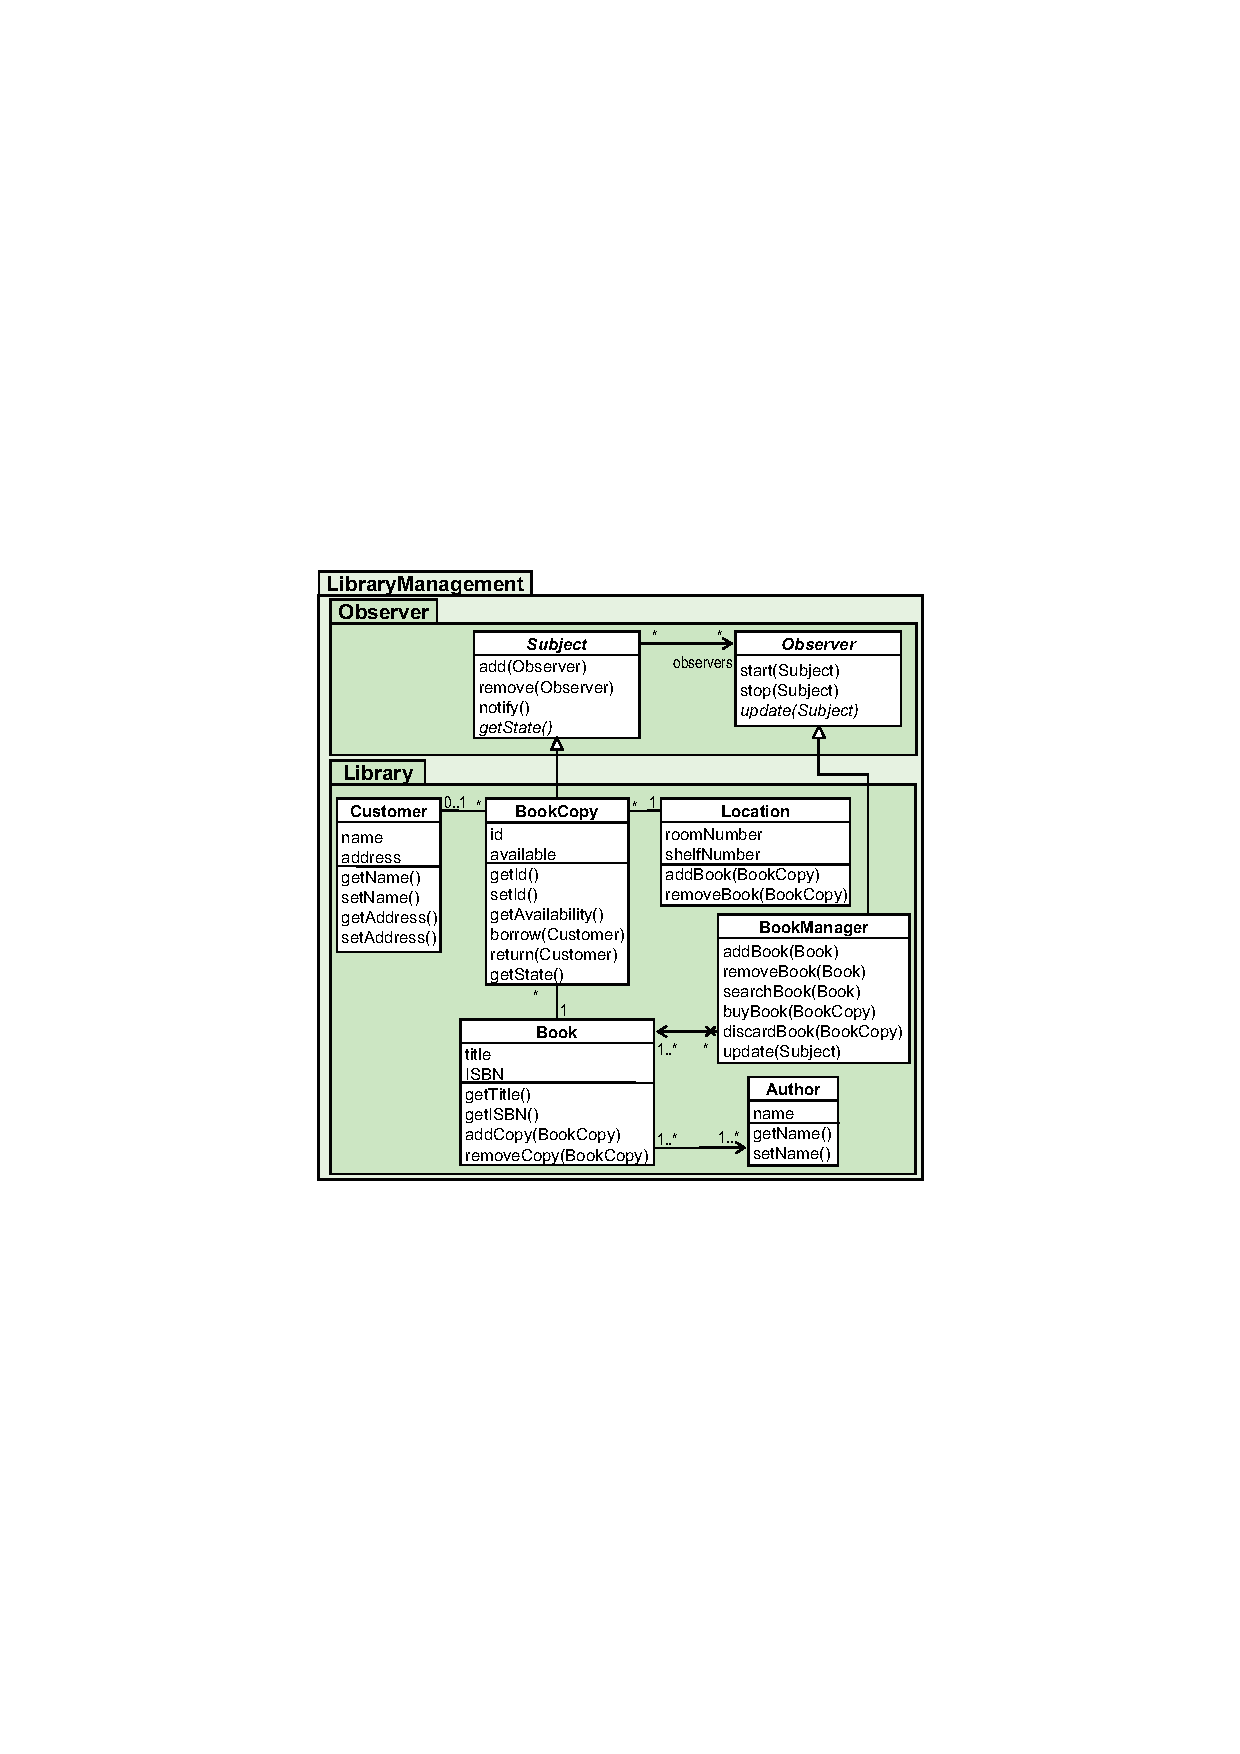
\includegraphics[width=0.7\textwidth]{chapters/figures/figure1}
	\caption{Sample figure}
	\label{fig:samplefigure_pdf}
\end{figure}


\section{Fonts}

When introducing important terms for the first time use \emph{emphasize}. For a consistent look and feel of proper names like {\cd} and {\uml{Observer}} pattern you may define macros in the main document \texttt{thesis.tex}.

\section{Code}

For short code fragments use the \textit{verbatim} environment.

\begin{verbatim}
//Start Program
System.out.println("Hello World!");
//End Program
\end{verbatim}

A much better alternative is the \textit{algorithm} environment (cf. Algorithm~\ref{alg:samplealgorithm}). This environment offers special formatting features for loops, operations and comments.

\begin{algorithm}[h!]
\SetKwData{Left}{left}
\SetKwData{This}{this}
\SetKwData{Up}{up}
\SetKwFunction{Union}{Union}
\SetKwFunction{FindCompress}{FindCompress}
\SetKwInOut{Input}{input}
\SetKwInOut{Output}{output}

\Input{A bitmap $Im$ of size $w\times l$}
\Output{A partition of the bitmap}

\BlankLine

\emph{special treatment of the first line}\;
\For{$i\leftarrow 2$ \KwTo $l$}{
\emph{special treatment of the first element of line $i$}\;
\For{$j\leftarrow 2$ \KwTo $w$}{\label{forins}
\Left$\leftarrow$ \FindCompress{$Im[i,j-1]$}\;
\Up$\leftarrow$ \FindCompress{$Im[i-1,]$}\;
\This$\leftarrow$ \FindCompress{$Im[i,j]$}\;
\If(\tcp*[r]{O(\Left,\This)==1}){\Left compatible with \This}{\label{lt}
\lIf{\Left $<$ \This}{\Union{\Left,\This}}\;
\lElse{\Union{\This,\Left}\;}
}
\If(\tcp*[r]{O(\Up,\This)==1}){\Up compatible with \This}{\label{ut}
\lIf{\Up $<$ \This}{\Union{\Up,\This}}\;
\tcp{\This is put under \Up to keep tree as flat as possible}\label{cmt}
\lElse{\Union{\This,\Up}}\tcp*[r]{\This linked to \Up}\label{lelse}
}
}
\lForEach{element $e$ of the line $i$}{\FindCompress{p}}
}
\caption{Sample algorithm}\label{alg:samplealgorithm}
\end{algorithm}



%%%%%%%%%%%%%%%%%%%%%%%%%%%%%%%%%%%%%%%%%
%%%   SELECT LANGUAGE    %%%%%%%%%%%%%%%%
%%%%%%%%%%%%%%%%%%%%%%%%%%%%%%%%%%%%%%%%%
% results in "Inhaltsverzeichnis", "Kapitel", "Abbildung", or "Contents", "Chapter", and "Figure"
\selectlanguage{english}
%\selectlanguage{ngerman} % files that use umlaut characters (ä,ö,ü) need to be encoded in utf-8


%%%%%%%%%%%%%%%%%%%%%%%%%%%%%%%%%%%%%%%%%
%%%   CONTENTS    %%%%%%%%%%%%%%%%%%%%%%%
%%%%%%%%%%%%%%%%%%%%%%%%%%%%%%%%%%%%%%%%%
\setcounter{tocdepth}{1}
\cleardoublepage
\pagestyle{numberCorner}
\tableofcontents*

%%%%%%%%%%%%%%%%%%%%%%%%%%%%%%%%%%%%%%%%%
%%%   MAINMATTER    %%%%%%%%%%%%%%%%%%%%%
%%%%%%%%%%%%%%%%%%%%%%%%%%%%%%%%%%%%%%%%%
\mainmatter
\pagenumbering{arabic}
\pagestyle{numberCorner}

%%%%%%%%%%%%%%%%%%%%%%%%%%%%%%%%%%%%%%%%%%
%\chapter{Introduction}
%\label{ch:intro}
%%%%%%%%%%%%%%%%%%%%%%%%%%%%%%%%%%%%%%%%%%
%
%\ifthenelse{\equal{\tuinfthesistype}{master}}
%  {\section{General Information}

This document is intended as a template and guideline and should support the author in the course of doing the master's thesis.
Assessment criteria comprise the quality of the theoretical and/or practical work as well as structure, content and wording of the written master's thesis. Careful attention should be given to the basics of scientific work (e.g., correct citation).

\section{Organizational Issues}

A master's thesis at the Faculty of Informatics has to be finished within six months. During this period regular meetings between the advisor(s) and the author have to take place.
In addition, the following milestones have to be fulfilled:
\begin{enumerate}
  \item  Within one month after having fixed the topic of the thesis the master's thesis proposal has to be prepared and must be accepted by the advisor(s). The master's thesis proposal must follow the respective template of the dean of academic affairs. Thereafter the proposal has to be applied for at the deanery. The necessary forms may be found on the web site of the Faculty of Informatics. \url{http://www.informatik.tuwien.ac.at/dekanat/formulare.html}
  \item  Accompanied with the master's thesis proposal, the structure of the thesis in terms of a table of contents has to be provided.
  \item Then, the first talk has to be given at the so-called ``Seminar for Master Students''. The slides have to be discussed with the advisor(s) one week in advance. Attendance of the ``Seminar for Master Students'' is compulsory and offers the opportunity to discuss arising problems among other master students.
  \item At the latest five months after the beginning, a provisional final version of the thesis has to be handed over to the advisor(s).  
  \item As soon as the provisional final version exists, a first poster draft has to be made. The making of a poster is a compulsory part of the ``Seminar for Master Students'' for all master studies at the Faculty of Informatics. Drafts and design guidelines can be found at \url{http://www.informatik.tuwien.ac.at/studium/richtlinien}.
  \item After having consulted the advisor(s) the second talk has to be held at the ``Seminar for Master Students''.
  \item At the latest six months after the beginning, the corrected version of the master's thesis and the poster have to be handed over to the advisor(s).
  \item After completion the master's thesis has to be presented at the ``epilog''. For detailed information on the epilog see: \\ \url{http://www.informatik.tuwien.ac.at/studium/epilog}
\end{enumerate}

\section{Structure of the Master's Thesis}

If the curriculum regulates the language of the master's thesis to be English (like for ``Business Informatics''), the thesis has to be written in English. Otherwise, the master's thesis may be written in English or in German. The structure of the thesis is predetermined.
The table of contents is followed by the introduction and the main part, which can vary according to the content. The master's thesis ends with the bibliography (compulsory) and the appendix (optional).

\begin{itemize}
  \item	Cover page
  \item Acknowledgements
  \item Abstract of the thesis in English and German
  \item Table of contents
  \item Introduction
  	\begin{itemize}
  		\item motivation
  		\item problem statement (which problem should be solved?)
  		\item aim of the work
  		\item methodological approach
  		\item structure of the work
  	\end{itemize}
  \item State of the art / analysis of existing approaches
  	\begin{itemize}
  		\item literature studies
  		\item analysis
  		\item comparison and summary of existing approaches
  	\end{itemize}
  \item Methodology
  	\begin{itemize}
  		\item used concepts
  		\item methods and/or models
  		\item languages
  		\item design methods
  		\item data models
  		\item analysis methods
  		\item formalisms
  	\end{itemize}
  \item Suggested solution/implementation
  \item Critical reflection
  	\begin{itemize}
  		\item comparison with related work
  		\item discussion of open issues
  	\end{itemize}
  \item Summary and future work
  \item Appendix: source code, data models, \dots
  \item Bibliography
\end{itemize}

}
%	{\section{General Information}

This document is intended as a template and guideline and should support the author in the course of doing the bachelor's thesis.
Assessment criteria comprise the quality of the theoretical and/or practical work as well as structure, content and wording of the written bachelor's thesis. Careful attention should be given to the basics of scientific work (e.g., correct citation).

\section{Structure of the Bachelor's Thesis}

If the curriculum regulates the language of the bachelor's thesis to be English, the thesis has to be written in English. Otherwise, the bachelor's thesis may be written in English or in German.
The table of contents is followed by the introduction and the main part, which can vary according to the content. The bachelor's thesis ends with the bibliography (compulsory) and the appendix (optional).

\begin{itemize}
  \item	Cover page
  \item Acknowledgments
  \item Abstract of the thesis in English and German
  \item Table of contents
  \item Introduction
  	\begin{itemize}
  		\item motivation
  		\item problem statement (which problem should be solved?)
  		\item aim of the work
  		\item methodological approach
  		\item structure of the work
  	\end{itemize}
  \item State of the art / analysis of existing approaches
  	\begin{itemize}
  		\item literature studies
  		\item analysis
  		\item comparison and summary of existing approaches
  	\end{itemize}
  \item Methodology
  	\begin{itemize}
  		\item used concepts
  		\item methods and/or models
  		\item languages
  		\item design methods
  		\item data models
  		\item analysis methods
  		\item formalisms
  	\end{itemize}
  \item Suggested solution/implementation
  \item Critical reflection
  	\begin{itemize}
  		\item comparison with related work
  		\item discussion of open issues
  	\end{itemize}
  \item Summary and future work
  \item Appendix: source code, data models, \dots
  \item Bibliography
\end{itemize}

}
%
%%%%%%%%%%%%%%%%%%%%%%%%%%%%%%%%%%%%%%%%%%
%\chapter{Typographic Design}
%\label{ch:typo}
%%%%%%%%%%%%%%%%%%%%%%%%%%%%%%%%%%%%%%%%%%

%% define custom macros for specific formats or names
\newcommand{\uml}[1]{\texttt{#1}}
\newcommand{\cd}{\textsf{Class Diagram}}

For working with \LaTeX you can take advantage of a variety of books and free introductions and tutorials on the internet. A competent contact point for \LaTeX beginners is the \LaTeX Wikibook, which is available under \url{http://en.wikibooks.org/wiki/LaTeX}. 

The following sections give examples of the most important \LaTeX environments and commands.

\section{Tables}

Tables have to be realized with the help of the \textit{table} environment. Tables shall be sequentially numbered for each chapter and described in terms of a short caption (cf. Table~\ref{tab:diplomaseminar}).

\begin{table}[htb]
	\centering
	\begin{tabular}{|l|c|c|}
		\hline \textbf{Name} & \textbf{Date} & \textbf{Title} \\
		\hline
		\hline Mustermann Adam  & 18.5   & T1    \\
		\hline Musterfrau Eva  & 22.6   & T2    \\
		\hline
	\end{tabular}
	\caption{Seminar for Master Students}
	\label{tab:diplomaseminar}
\end{table}


\section{Figures}

Like tables, figures shall be sequentially numbered for each chapter and described in terms of a short caption). You could either produce your drawings directly inside \LaTeX using PSTricks\footnote{\url{http://tug.org/PSTricks}}, Tikz\footnote{\url{http://sourceforge.net/projects/pgf}}, or any set of macros dedicated to your requirements (cf. Figure~\ref{fig:samplefigure_tikz}). Alternatively, you may include figures prepared in external tools (cf. Figure~\ref{fig:samplefigure_pdf}). Note, to ensure high quality printing, all figures must have at least 300 dpi.

\begin{figure}
	\centering
	\begin{tikzpicture}[->, auto, node distance=2.8cm, semithick]
	  \node[initial, state] (1)		 {$S_1$};
	  \node[state] 		(2) [right of=1] {$S_2$};
	
	  \path (1) edge [bend left]  node {0} (2)
		(1) edge [loop above] node {1} (1)
		(2) edge [bend left]  node {0} (1)
		(2) edge [loop above] node {1} (2);
	\end{tikzpicture}
	\caption{Sample figure}
	\label{fig:samplefigure_tikz}
\end{figure}

\begin{figure}[tb]
	\centering
	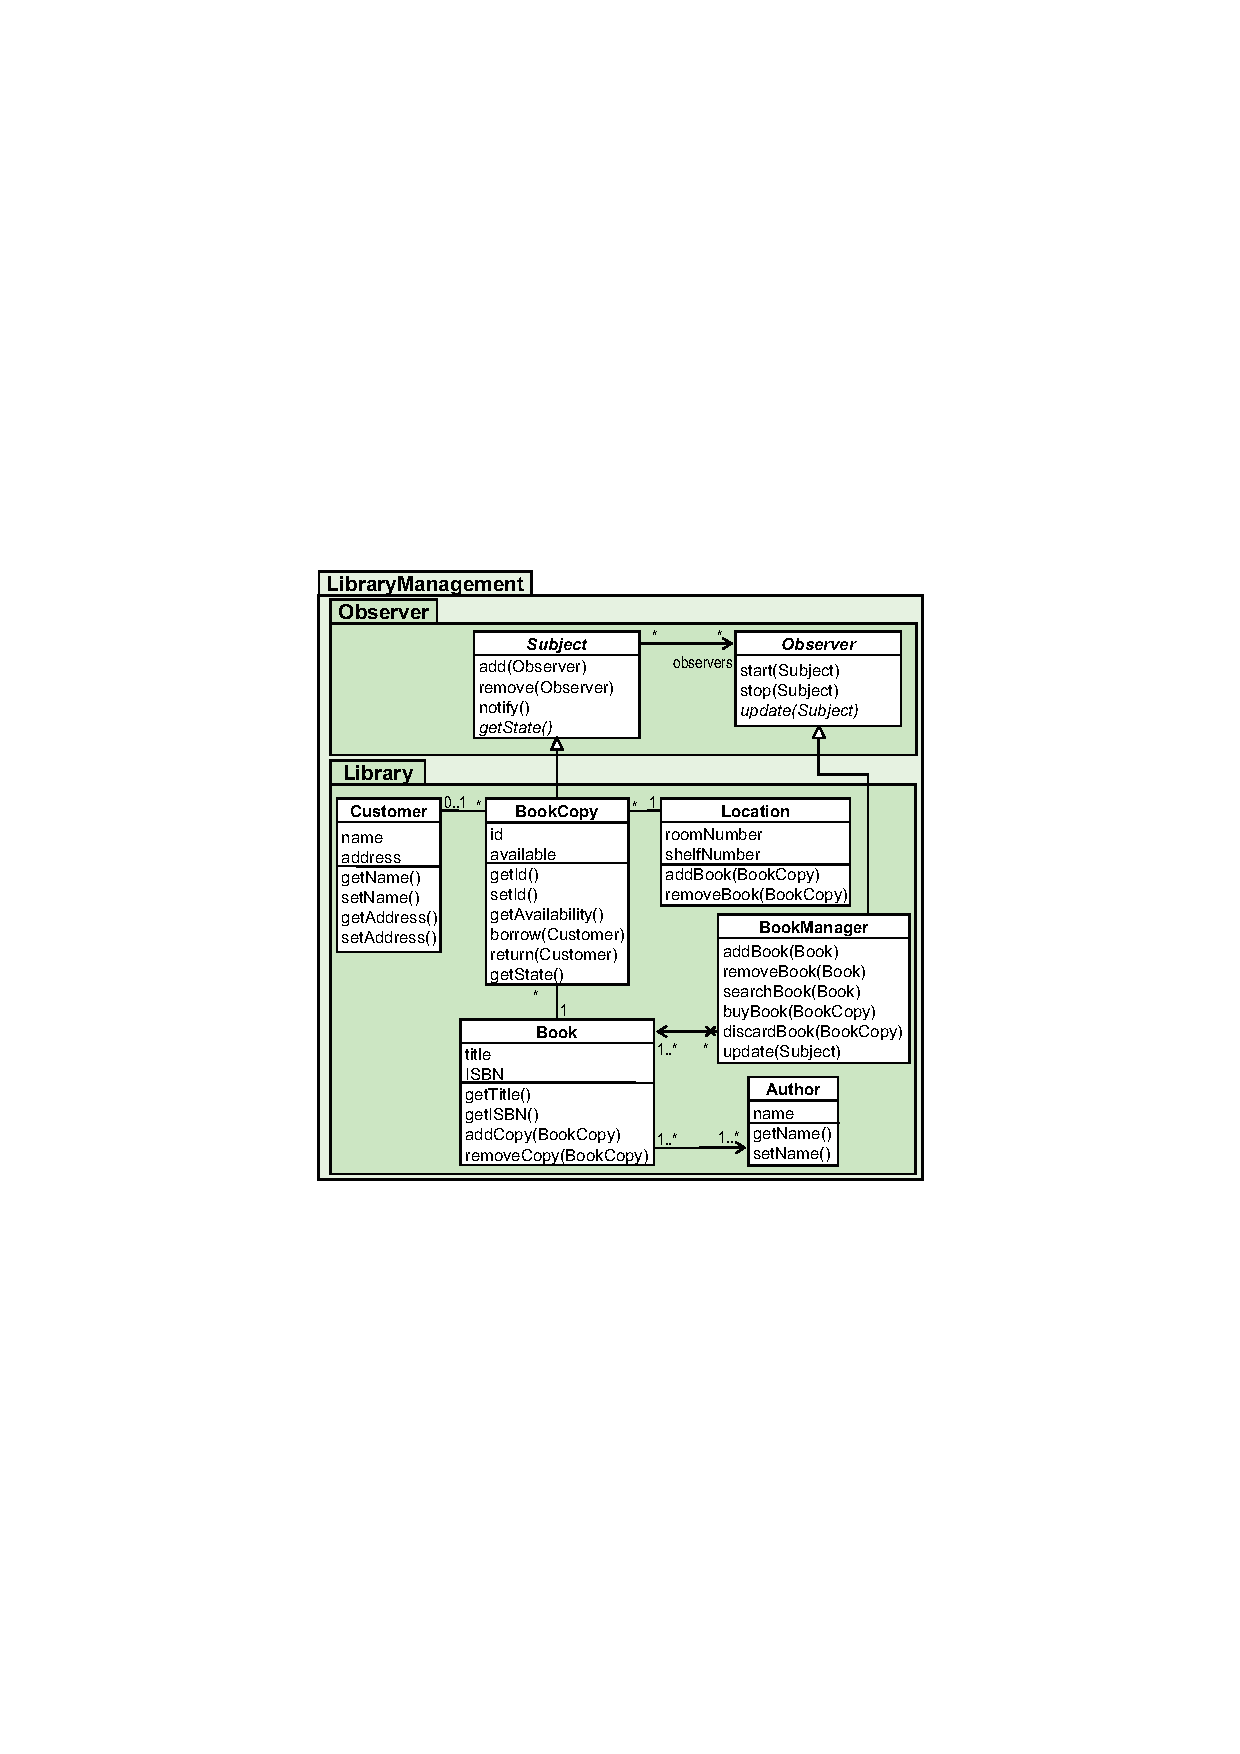
\includegraphics[width=0.7\textwidth]{chapters/figures/figure1}
	\caption{Sample figure}
	\label{fig:samplefigure_pdf}
\end{figure}


\section{Fonts}

When introducing important terms for the first time use \emph{emphasize}. For a consistent look and feel of proper names like {\cd} and {\uml{Observer}} pattern you may define macros in the main document \texttt{thesis.tex}.

\section{Code}

For short code fragments use the \textit{verbatim} environment.

\begin{verbatim}
//Start Program
System.out.println("Hello World!");
//End Program
\end{verbatim}

A much better alternative is the \textit{algorithm} environment (cf. Algorithm~\ref{alg:samplealgorithm}). This environment offers special formatting features for loops, operations and comments.

\begin{algorithm}[h!]
\SetKwData{Left}{left}
\SetKwData{This}{this}
\SetKwData{Up}{up}
\SetKwFunction{Union}{Union}
\SetKwFunction{FindCompress}{FindCompress}
\SetKwInOut{Input}{input}
\SetKwInOut{Output}{output}

\Input{A bitmap $Im$ of size $w\times l$}
\Output{A partition of the bitmap}

\BlankLine

\emph{special treatment of the first line}\;
\For{$i\leftarrow 2$ \KwTo $l$}{
\emph{special treatment of the first element of line $i$}\;
\For{$j\leftarrow 2$ \KwTo $w$}{\label{forins}
\Left$\leftarrow$ \FindCompress{$Im[i,j-1]$}\;
\Up$\leftarrow$ \FindCompress{$Im[i-1,]$}\;
\This$\leftarrow$ \FindCompress{$Im[i,j]$}\;
\If(\tcp*[r]{O(\Left,\This)==1}){\Left compatible with \This}{\label{lt}
\lIf{\Left $<$ \This}{\Union{\Left,\This}}\;
\lElse{\Union{\This,\Left}\;}
}
\If(\tcp*[r]{O(\Up,\This)==1}){\Up compatible with \This}{\label{ut}
\lIf{\Up $<$ \This}{\Union{\Up,\This}}\;
\tcp{\This is put under \Up to keep tree as flat as possible}\label{cmt}
\lElse{\Union{\This,\Up}}\tcp*[r]{\This linked to \Up}\label{lelse}
}
}
\lForEach{element $e$ of the line $i$}{\FindCompress{p}}
}
\caption{Sample algorithm}\label{alg:samplealgorithm}
\end{algorithm}


\chapter{Introduction}
\section{Illustration}
\begin{quote}
``The aim of illustration is to generate expressive images that effectively convey certain information via the visual channel to the human observer.'' \cite{Viola:2005:SVV:2381219.2381249}
\end{quote}

Illustrations have been used since the paleolithic age\cite{Viola:2005:SVV:2381219.2381249} to give their viewers a graphical representation of things seen, experienced or imagined. Since the development of perspective and the necessity to intuitively explain complex technical, medical and scientific matters, especially since the industrial revolution, several techniques to successfully achieve this have been developed.
\begin{quote}
``Illustrative techniques are often designed in a way that even a person with no technical understanding clearly understands the piece of art.'' \cite{Viola:2005:SVV:2381219.2381249}
\end{quote}
With the arrival of computers that are able to create complex graphics that react in real-time to user interactions, the transfer of these static illustrations to a dynamic visual representation has posed new challenges to the art of illustration.\\

\section{Exploded view and ghosting}
The exploded view is a technique used in illustrative visualization, where complex real world objects are drawn in a way that conveys how these objects are built, how they are assembled or how they work. Typically these objects are systems of interacting parts that may occlude each other or even be completely hidden by an outer hull of the visualized objects.\\
Examples for this would be a motor that consists of many independent parts, where the Illustration should give an idea of how it might work, a chest of drawers bought as a set of boards and connectors, that has a visual assembly instruction or the depiction of an anatomic feature.\\
\begin{quote}
``In an exploded view the object is decomposed into several parts which are displaced so that internal details are visible'' \cite{proc:bruckner-2006-EVV}
\end{quote}
For technical illustrations the parts that constitute a machine could be moved on an axis so that they are all visible and their position relative to this axis would still give information as to where the place of each part would be inside the machine. As for the assembly instruction the displacement would happen along the axes they will be put together to make it clear to the viewer how to assemble the object.\\
The goal of my work was to create an interactive visualization that would dynamically generate simple exploded views. Building upon an existing plugin for the VolumeShop visualization platform, that splits objects along a plane and displaces the two parts,  I created a plugin where the user can define an object of interest, that is not cut and stays in place, while the split parts are displaced, revealing said object.\\
The visualization system is interactive, the User can also choose, which part of the system is interesting to him, and view the object from different angles. From each perspective and foreach object of interest the system has to ensure that the object of interest is visible, the resulting visualization is compact but not too cluttered.  Because of this the ideal position of the exploded parts is constantly shifting upon interaction. To give the transitions a more natural and therefore aesthetically pleasing look this displacement- the ''explosion''- can be shown as an animation.\\
When looking from a direction close to the displacement axis, the explosion distance becomes so large, that the object of interest is either to small, because it's to far away when the whole graphic is displayed or parts of the graphic missing becuse they are behind the camera.
To prevent this, I designed a system with a maximum distance of displacement. Now the exploded parts occlude the object of interest when viewing from a critical direction. To be able to show the object of interest nevertheless I combined the exploded view with ghosting, which is a different illustration technique where objects that are occluding other objects are being drawn transparently. \ref{fig:demo}\\
\begin{figure}[tb]
	\centering
	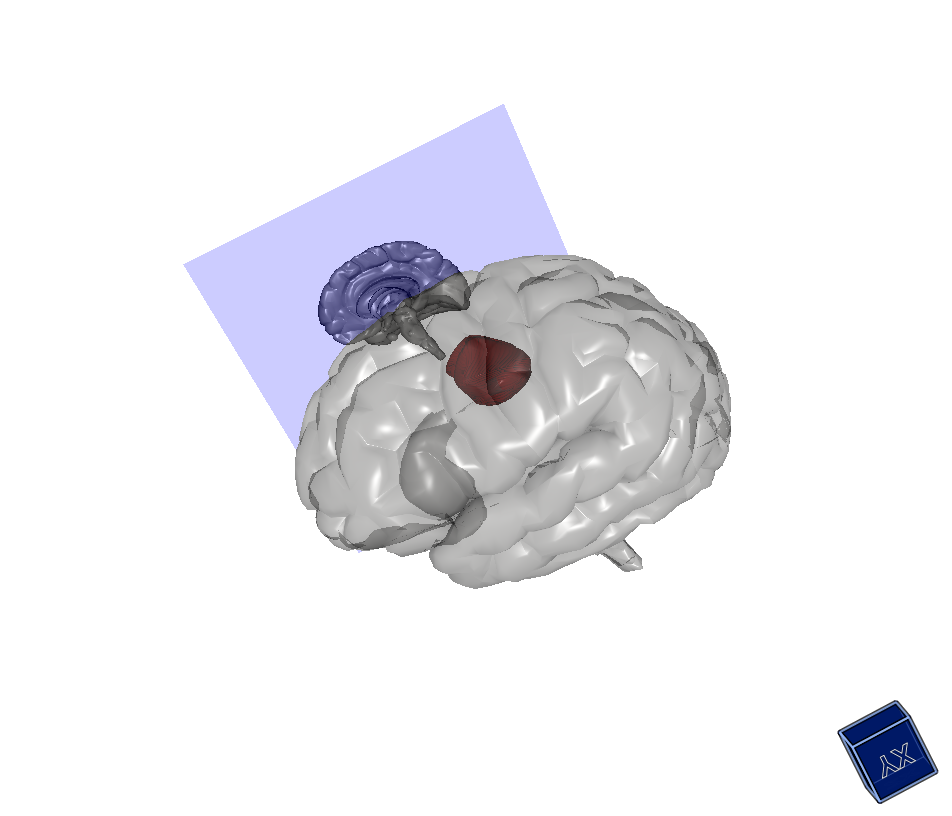
\includegraphics[width=0.7\textwidth]{chapters/figures/demo}
	\caption{Illustration of a brain, combining ghosting and an exploded view}
	\label{fig:demo}
\end{figure}
\chapter{Related Work}

\begin{wrapfigure}{r}{0.3\textwidth}
  \begin{center}
    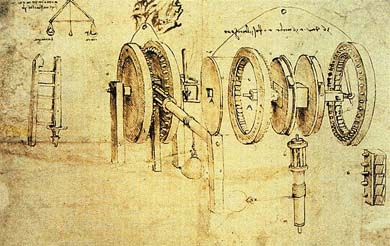
\includegraphics[width=0.28\textwidth]{chapters/figures/davinci}
  \end{center}
  \caption{Exploded view by Leonardo da Vinci}
  \label{fig:davinci}
\end{wrapfigure}
Like many other techniques exploded views by themselves are nothing new, hand-drawn and -designed instances of this technique have existed since the rennaissance (see \ref{fig:davinci}). 
\begin {quote}
They (illustrators) carefully choose the size and shape of cuts, as well as the placement of the parts relative to one another, to expose and highlight the internal structure and spatial relationships between parts.\cite{Agrawala:2011:DPV:1924421.1924439}
\end{quote}
Agrawala et al. \cite{Agrawala:2011:DPV:1924421.1924439} describe methods of how to generally create and evaluate design principles for visual communication: by analyzing existing examples of a technique, analyzing them using insights from cognitive and perceptive science, design rules are hypothesized. These design priciples are often qualitative guidelines and can not be simply translated into a generative algorith. They are then to be evaluated by user feedback from making the visualization available to the public and user studies.\\
\section{What are the main challenges when creating exploded views?}
For the concrete problem of creating exploded views Li et al.\cite{proc:Li:2008:AGI} provide a comprehensive list of such guidelines and what the challenges of the process of implementing them in an interactive system are.\\
Most important of all is the question what information should be communicated with the image and what the purpose of the illustration is. In essence what are the objects of interest that should attract the viewers attention? This usually is determined by preliminary definition of interesting features, definitions of parts, subsets of parts of the data or user interaction while viewing the graphic.
\subsection{Explosion direction}
Also one has to consider in which direction the parts should be displaced. 
\begin{quote}
Many objects have a canonical coordinate frame that may be defined by a number of factors, including symmetry , real-world orientation, and domain-specific conventions. In most exploded views, parts are exploded only along these canonical axes.\cite{proc:Li:2008:AGI}
\end{quote}
Especially if the graphic conveys technical instructions or how-things-work-descriptions descriptions these axes are usually the directions in which they are assembled \cite{Agra03} or - if applicable- the axis around which they rotate\cite{MitraYYLA13}.
If the interesting parts are inside a container that is also part of the object, this container is split and its segments are also exploded. In the most simple approach, which is what I implemented, the cutting plane is the normal plane of the explosion direction, with the center of the object's bounding box (see \ref{fig:splitting}).
\begin{figure}[tb]
	\centering
	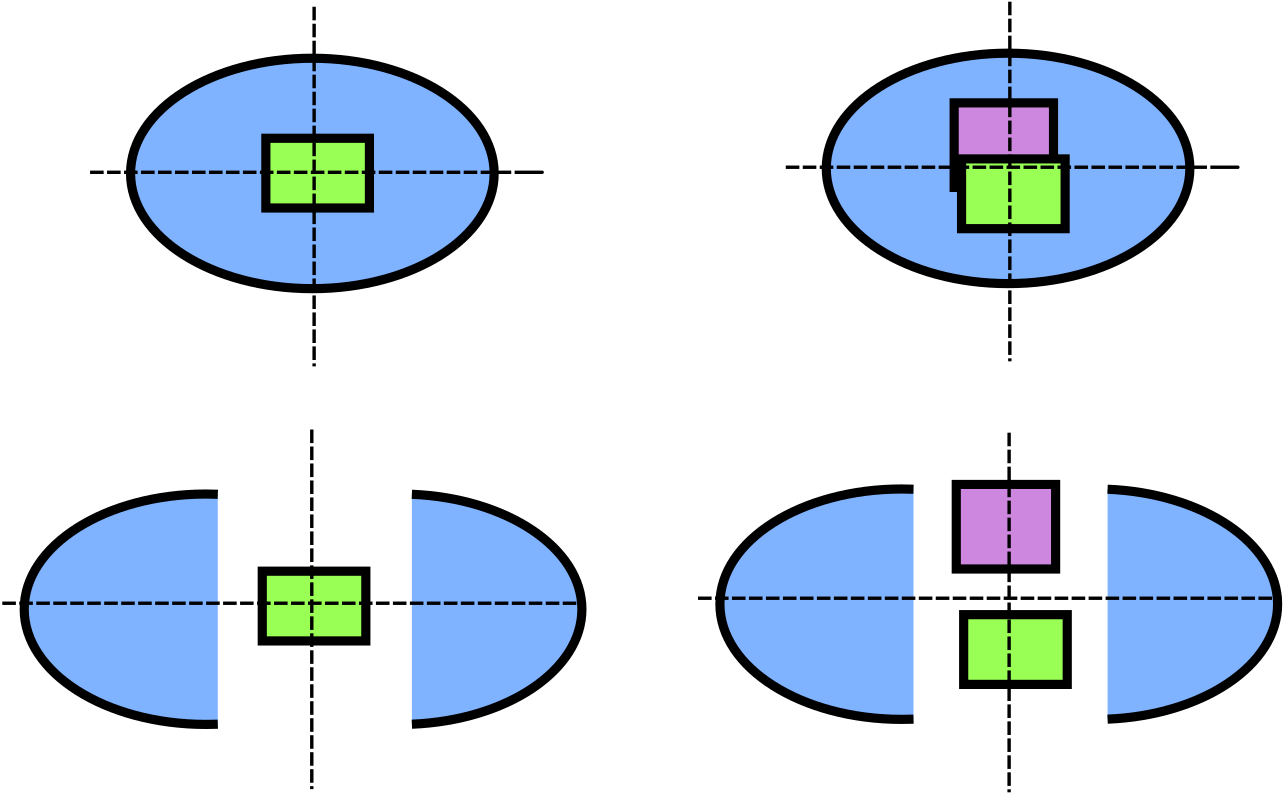
\includegraphics[width=0.9\textwidth]{chapters/figures/splitting}
	\caption{The object of interest is revealed by splitting its container and moving the two segments away from the object in the center.}
	\label{fig:splitting}
\end{figure}
\subsection{Part hierarchy}
Take for example an object that has a container and a lot of small parts that inside whose function should be clarified by exploding them in their canonical direction.  In this case it might be convenient to split and explode the container along a different axis than the internal parts to get a more compact visualization(see \ref{fig:axes}).\\
\begin{figure}[tb]
	\centering
	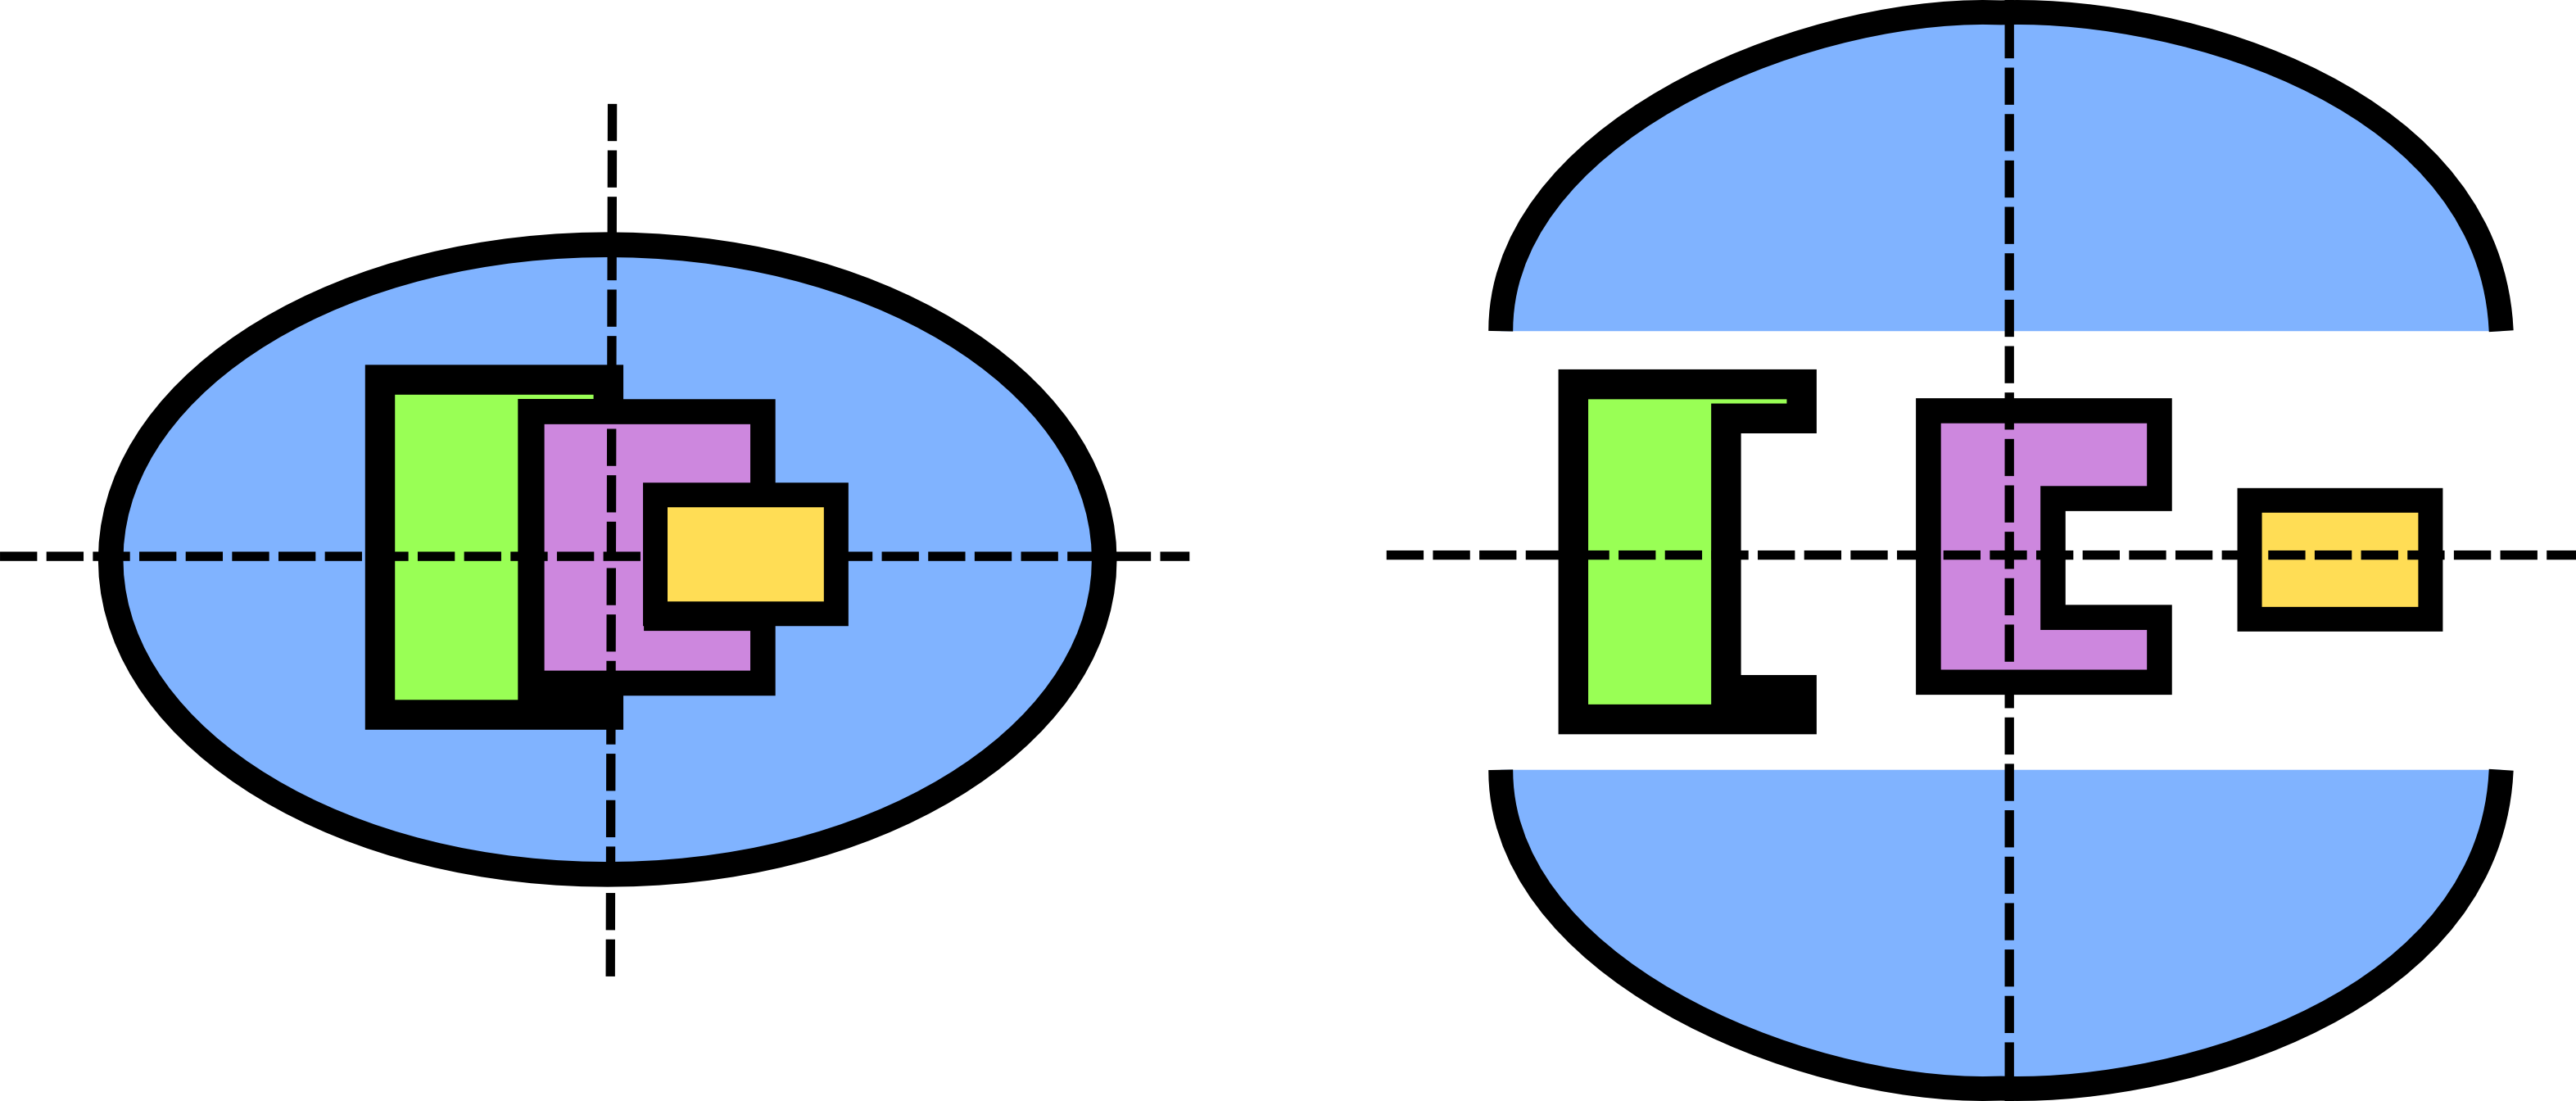
\includegraphics[width=0.7\textwidth]{chapters/figures/axes}
	\caption{The interior parts of an object are exploded in a different direction than their container}
	\label{fig:axes}
\end{figure}
In some cases, especially in the case technical visualizations e.g. assembly instructions or visual descriptions of machines the parts would block each other if they are not disassembled in the correct order and direction. A solution for this is an explosion graph representation of the Object\cite{proc:Li:2008:AGI}: Each node of this directional acyclic graph has edges pointing to parts blocking it from exploding (see \ref{fig:hierarchy}). It is generated by an algorithm, that, starting with all parts in the active set, would recursively check for unblocked parts,remove them from the active set and draw an edge from the unblocked part to any active part that would touch it.\\
To further expand the possibilities, several parts can be grouped into sub-assemblies that are then part of a hierarchical explosion graph. that has explosion graphs as nodes.\\
\begin{figure}[tb]
	\centering
	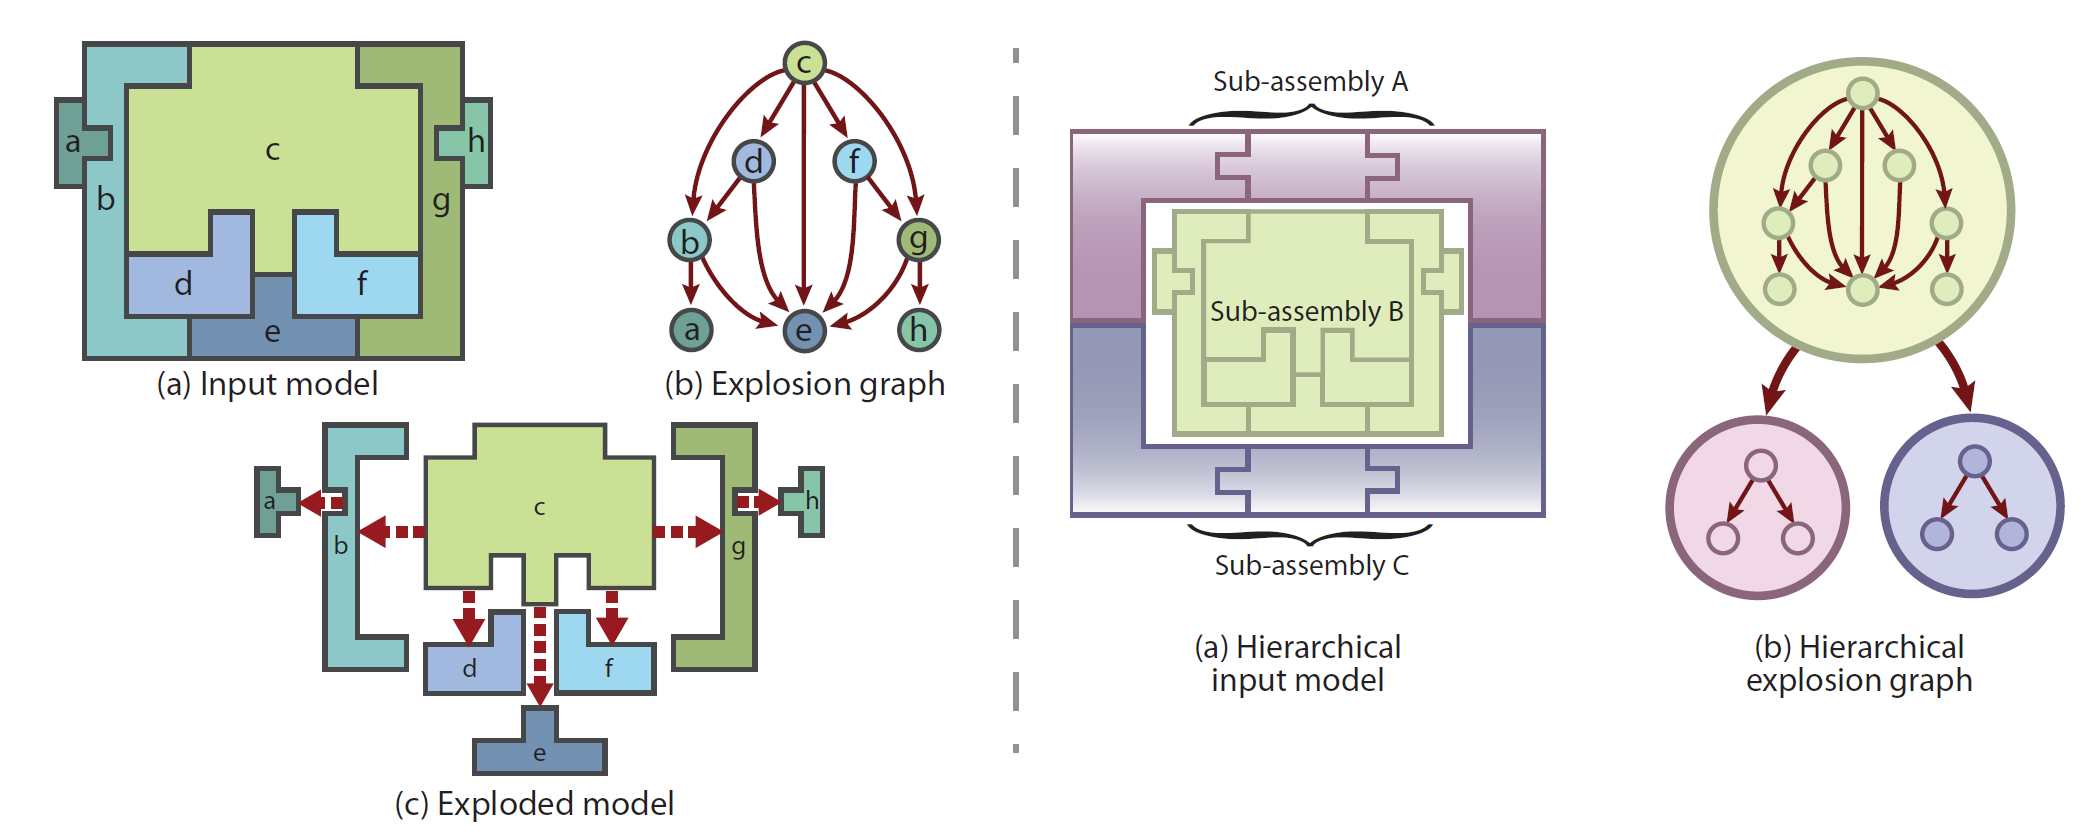
\includegraphics[width=0.7\textwidth]{chapters/figures/hierarchy}
	\caption{Explosion graph and hierarchical explosion graph\cite{proc:Li:2008:AGI}}
	\label{fig:hierarchy}
\end{figure}
If one now wanted to see a certain part of the object of interest in an exploded view, all of the parts that its edges in the explosion graph point to would have to be exploded first. If it were also part of a sub-assembly, all sub-assemblies that would have edges pointing from the part's subassembly would need to be exploded before that.
\subsection{Visibility}
Another challenge is the decision how far to displace the objects. Ideally each part should be fully visible but if there are many objects to be exploded or system the displacement direction is similar to the viewing direction, the size of the graph would grow to be enormous therefore resulting in loss of detail and expressiveness of the visualization. That may make it necessary to have some overlap as a trade-off to retain the compactness of the visualization.\\
\begin{figure}[tb]
	\centering
	\includegraphics[width=0.9\textwidth]{chapters/figures/perspective}
	\caption{The closer the viewpoint comes to the displacement axis, the larger has to be the offset to reveal the whole object of interest}
	\label{fig:perspective}
\end{figure}
With a freely rotatable and movable viewpoint the user can avoid visual clutter or lack of compactness (depending on how the system behaves) by choosing a viewpoint that provides as little clutter as possible,which narrows down the possibilities of expressive viewpoints to a minimum.\\
A solution for this would be to use a view dependent force-based displacement behavior as suggested by Bruckner and Gr\"oller\cite{proc:bruckner-2006-EVV}: Each exploding part is being displaced by a sum of multiple forces:
\begin{itemize}
\item \textbf{Explosion force} This force is pushing the part away from its original location, its magnitude is indirectly proportional to $e^{||r||}$ where $r$ is the distance between the object and the explosion point
\item \textbf{Spacing force} This repulsive force that each exploded part effects on all other exploded parts prevents parts from clustering and is indirectly proportional to $r^2$ where $r$ is the distance between the two parts.
\item \textbf{Viewing force}Additionally,  a viewing force is introduced that pushes the parts away from the viewing ray, thus preventing occlusions. It is indirectly proportional to the distance $r$ between the viewing ray and the part.
\end{itemize}
\begin{figure}[tb]
	\centering
	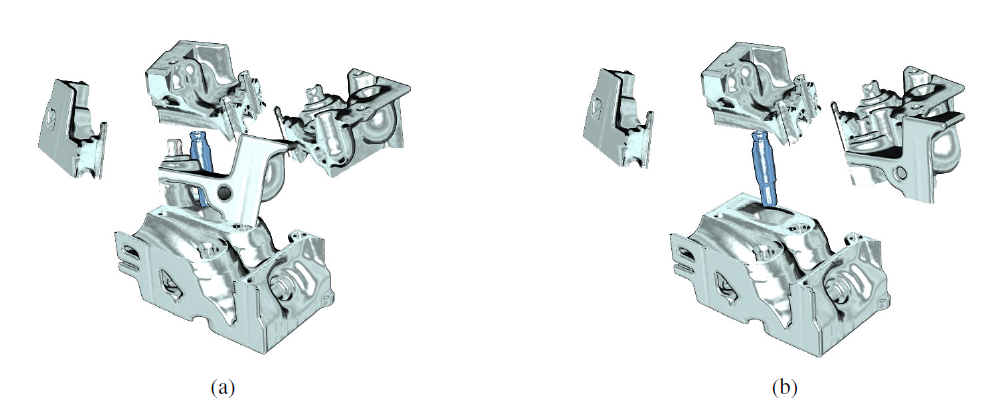
\includegraphics[width=0.7\textwidth]{chapters/figures/motor}
	\caption{(a) force-based exploded view without viewing force (interesting part is occluded) (b) with viewing force\cite{proc:bruckner-2006-EVV}}
	\label{fig:motor}
\end{figure}
This approach results in very intuitive manipulation of the graphic, making the part of the object of interest that one is looking at always visible with smooth transitions between the positions of the parts when changing viewpoints.\\
In this approach the parts don't have to explode along a predefined axis, the explosion direction can be dynamically determined by the forces, which looks impressive for anatomical data, for a technical illustration it is less desirable, for one of the key advantages of exploded views, the retention of information of a subpart's location in a system is partially lost without a clear displacement direction.\\
The solution presented in the paper is able to define axes along which to explode, this, though with similarly intuitive interaction by looking at a certain point still has the problem of little oversight when viewing from certain angles.
\subsection{Elxploded views in architectural visualization}
In architecture the need to visually communicate complex ideas about what a building should look like are essential to the craft. Exploded views are one of the techiques employed for this, in many shopping malls or complex public buildings(e.g. TU Wien) the floor plans are simple exploded views of teh building. Niederauer et al. \cite{TODO} have devised an interesting non-invasive method to achieve this kind of floor layout:\\
First a possible candidate for a splitting plane needs to be found, ideally this is the ceiling of a floor.
By counting the number of downward facing poligons at each possible vertex height, and define those heights with an exceptionally large number of downward facing poligons as a ceiling of  floor. They then split and displace the meshes upwards until everything is visible, which results in an exploded view of the architecture that was analized. The most intriguing thing is that they do that by manipulating the openGL output Stream of third party software (among others Quake III) without the need to change that software in any way.\\
Fleiss \cite{TODO} aproaches a similar problem though not just limited to drawing a foor plan with only one explosion direction, but a complex view that aims to illustrate the layout of walls, roofs, etc.

SOME WORDS ABOUT THE GRAMMAR AND THE USER STUDY

\subsection{Ghosting}
As the exploded view, ghosting is a smart visibility technique to illustrate the normally occluded inner workings of a complex object. In this case smart visibility is defined like this.
\begin{quote}Smart Visibility considers more than just light propagation. For example also the relevance of the individual objects is taken into account. An important object might shine through an otherwise occluding object closer to the viewer. \cite{Viola-05-Smart}\end{quote}
The advantages of this technique are that the in contrast to the exploded view, objects visualized with ghosting do not take up more space than the objects themselves. Additionally, the inner parts of an object are shown at their actual position inside the object, thus being able to show the composition of an object accurately than an Exploded view might be able to do. Another advantage is that because the occluding object is not completely surpressed, \\
On the other Hand, ghosted views are usually more cluttered because of this, which can lead to loss of detail and insight. Also they tend to look confusing in case two objects are in between the viewer and the object of interest. To avoid these problems and achieve good results the following rules should be considered:\cite{Viola-05-Smart}
\begin{itemize}
\item faces of transparent objects never shine through
\item objects occluded by two transparent objects do not shine through
\item transparency falls off close to the edges of transparent objects
\end{itemize}
\subsection{Interactivity}
The biggest advantage of a computerized illustration over the classic static illustration is interactivity, most obviously the possibility to view an object from every different direction, which as described above creates its own challenges. Another aspect is the possibility for the user to choose which part of the graphic are interesting to her or him.\\
 In Li et al.'s solution\cite{proc:Li:2008:AGI} this is restricted to the predefined parts of the data sets that can be selected by clicking on them which causes the explosion to adapt, so that the selected part is fully visible. Another possibility is dragging a part along its explosion axis which causes which causes all parts on that axis to move along with it until a part that moves along a different axis is encountered. Also a 3D fish-eye viewing technique can be used that, akin to the viewing force \cite{proc:bruckner-2006-EVV} can be used to move the parts along their axes.\\
The force-based solution is -due to the use of volume data- more flexible in the definition of parts that can be exploded: the data can be freely partitioned in cuboid subspaces that can be linked by hinges or to an axis, that can be exploded by the forces three above, each of which can be varied between a 0 and a maximum value along  with the degree of explosion\\



\chapter{Practical part}
The practical part of my thesis was to create a plug-in for the visualization application ``Volumeshop `` that was developed at the Computer graphics institute at TU Wien. I built my work upon an Existing plug-in, that split meshes in image space.
\section{Plan and milestone definition:}
The practical part was split into three milestones containing the following tasks:
\begin{itemize}
\item \textbf{Milestone 1} \emph{Selection of split meshes, selected parts are not split and stay in place} Make a simple, intuitive but manual way of creating exploded Views.
\item \textbf{Milestone 2} \emph{Find a safe distance, find a split plane} Automatize the creation of the visualization, by automatically finding a split plane and an offset.
\item \textbf{Milestone 3} \emph{Optimize Distance, force-field animation of split, optimize fringe distance cases} Make the visualization more pleasant to look at by adding a seemingly antural force-field animation and prevent unnecessary large offsets by introducing ghosting techniques.
\end{itemize}
\section {Tools and languages}
Since the project is based upon an existing framework, I used its languages, c++ for the main program and the GLSL for the openGL shaders.
\section{Documentation of the implementation each milestone}
\subsection{Milestone 1:Selection of split meshes, selected parts are not split and stay in place} The original plug-in drew split meshes by drawing them twice, with a manually defined offset, from a manually defined split plane. The fragment shader then rejects fragments that were behind or in front of the also translated split plane, rendering them in a predetermined fashion.\\
The first step towards an exploded view was now to use the already implemented group selection feature to define an object of interest that would not be split or translated like the rest of the mesh. To realize this I introduced a third rendering of the mesh in the display function. This render pass would render only the object of interest in its original location in the non-displaced mesh.\\
This also required that the ``renderMesh''-function be modified, introducing a new boolean parameter ``split'' that tspecifies, if the object is rendered in split mode, or in the ``object-of-interest-mode''. When the function loops through the groups of a mesh, it checks if the the group is in the group . If that is the case and the function parameter ``split'' is false, the group will be rendered. If split is false and the group is not selected, it will also be drawn, this time displaced.\\
Also a new option ``split'' for the shader was introduced, given that there is no need to pass an offset or split plane to render the object of interest. This basically reverts the fragment shader to the original trianglemesh-shader\\
After that was done an exploded view of the object was now rendered with manual definition of the offset and split plane with one usability glitch: A colour picking algorithm was already implemented, but it didn't consider the splitting and translation of the object. This resulted in a behaviour where clicking on a part of the object when it was split would cause false selection or deselection. \\
To set this right, I modified the the overlay function so that it would also be rendered three times like the normal rendering, modifying the ``renderGroup'' function once more  so that it could also render the overlay function and adding an ``overlay''option to the shader.
\begin{figure}[tb]
	\centering
	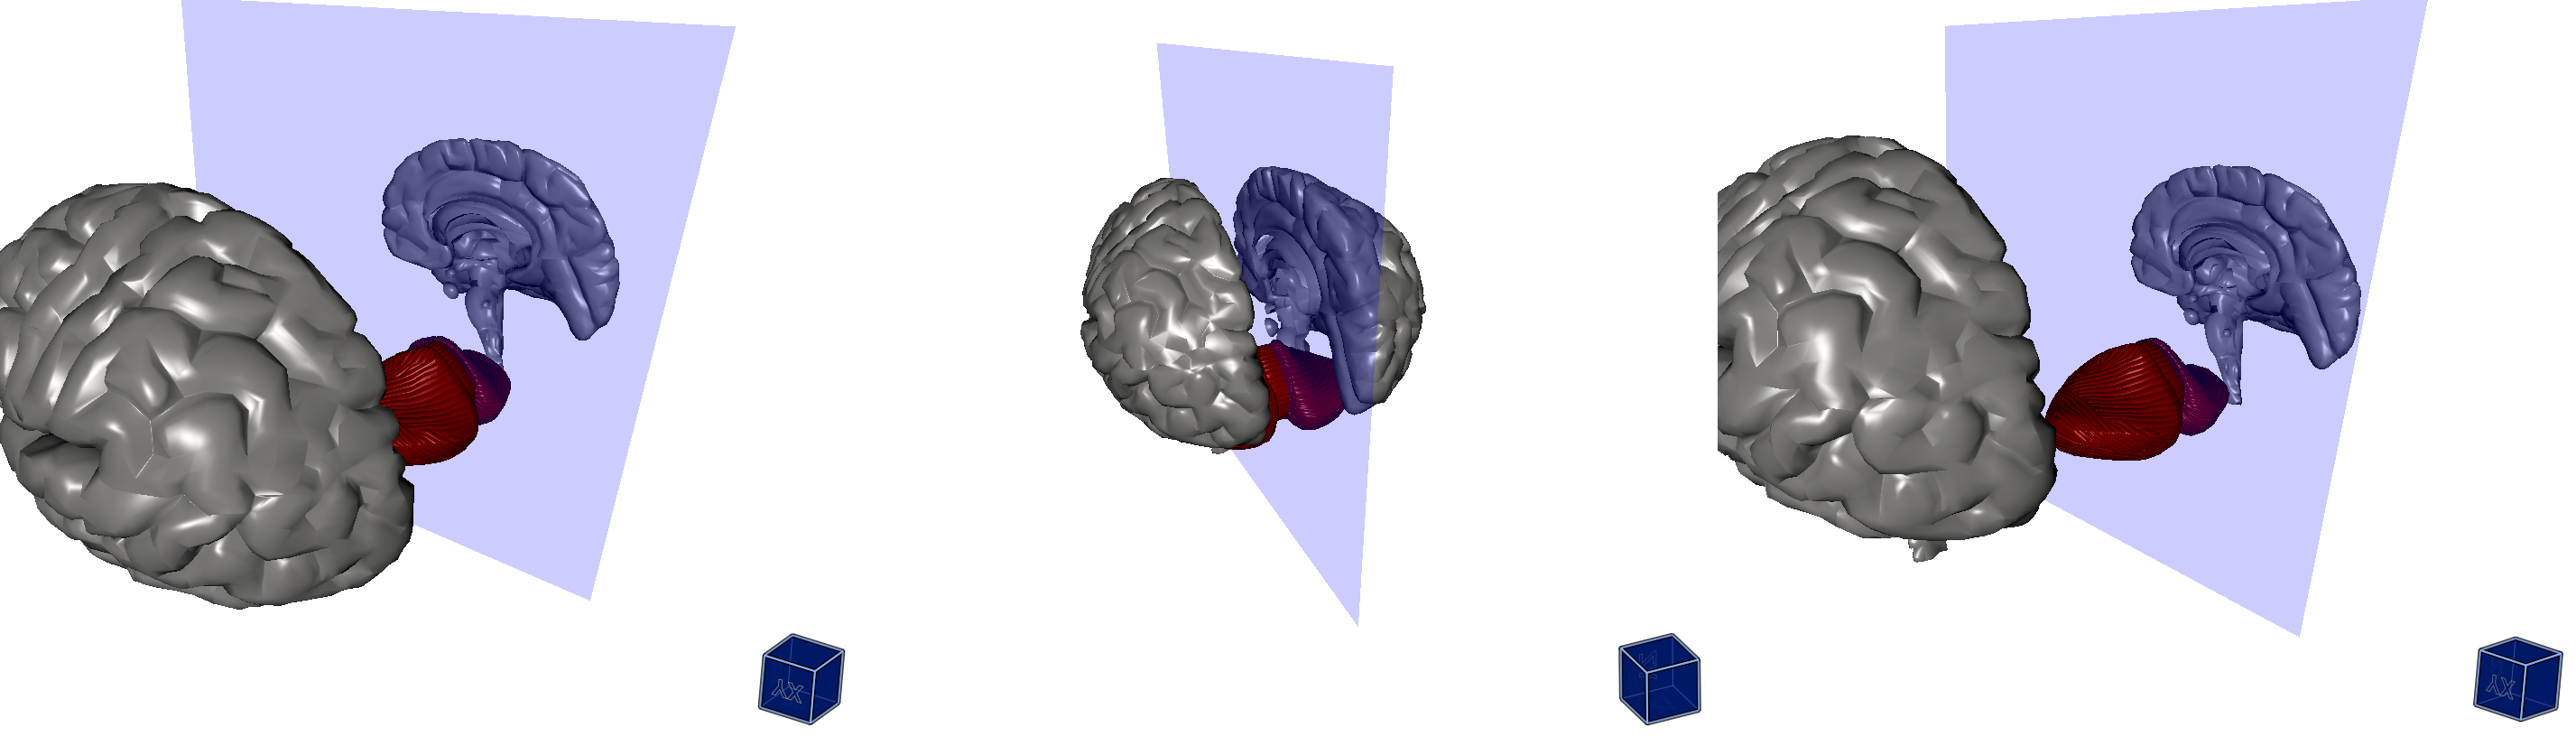
\includegraphics[width=0.9\textwidth]{chapters/figures/cerebellum}
	\caption{Exploded view of a brain with the offset of the displaced halves are set amanually}
	\label{fig:cerebellum}
\end{figure}

\subsection{Milestone 2: find a safe distance, find a split plane} 
The next step would be to automatically place the two halves of the object so that they would not collide with the object of interest and to find a suiting plane to split the object.\\
As I was aiming for an animated transition between offsets, I chose an implicit approach to finding the ideal offset of the two halves:\\
Each time the object would be rendered I would first render the three parts (Object of interest, front half, back half) with the low-cost overlay shader counting the rendered pixels of the non-occluded object ($p_{unoccluded}$), counting the amount of pixels drawn using openGL occlusion queries and during the actual rendering counting the amount of pixels drawn with possible occlusions ($p_{occluded}$). The ratio $r$ determined by
\begin{equation}\label{eq:Occlusion ratio}
	r =\frac{p_{unoccluded} - p_{occluded}}{ p_{unoccluded}}
\end{equation}
for
\begin{equation}
	p_{occluded} \neq 0
\end{equation}

is multiplied with the speed specified by user input resulting in the speed at which the offset grows toward an ideal offset which is the maximum offset described in Milestone 3 or an offset of 0 if the difference between  ($p_{unoccluded}$) and  ($p_{occluded}$) is 0 with the ideal offset different than the maximum offset.\\
Because the ratio tends towards 0 the more the object is revealed the growth of the offset diminishes the more is revealed , coming to a halt as soon as the whole object is fully revealed which is the moment the ideal offset is set to the current offset.\\
%\begin{verbatim}
%float ratio_selected = occlusions[0]- occlusions[1];
%	if (ratio_selected>0){
%	ratio_selected/=occlusions[0];
%	if (ghosting){
%		ideal_offset[0]=boundsDiameter;
%		ideal_offset[1]=-boundsDiameter;
%	}else{
%		ideal_offset[0]=20.0f;
%		ideal_offset[1]=-20.0f;
%	}
%	speed=GetPlugin().GetProperty("Speed");
%	speed*=ratio_selected;
%}else{
%	//stop
%	}
%\end{verbatim}
This movement is akin to the movement of the object being pulled by a spring toward the point of full revelation of the object of interest, though not a linear spring, because the change of speed is determined by the amount of Pixels that are revealed in each iteration making the spring constant proportional to $r$.
To avoid that the Object still moves at very low speeds, resulting in huge amounts of unnecesary costly redraws,I introduced a  minimum speed $\epsilon$ so that the object comes to a halt earlier.\\

\subsection{Milestone 3: Optimize Distance, force-field animation of split, optimize fringe distance cases} 

The objective of this last Milestone is to give a smooth appearance to the graphic while the view is changed by User interaction. The first step is to make the transition between two offsets smooth with the transition speed $s$ proportional to $\Delta_{offset}$
\begin{equation}
	s=s_u \cdot \Delta_{offset}
\end{equation}
thus creating a movement with linear deceleration that comes to a halt when the ideal offset is reached. this behaviour can be observed if the option ``Dynamic Offset `` is deactivated.\\
With dynamic ratio turned on and the object of interest is (partially) occluded the ideal offset is set to the maximum  offset and speed $s$ is multiplied by the ratio $r$ described in milestone 2 so that when the split parts move away from the object of interest the movement halts when the whole object is fully revealed setting the current offset as the ideal offset.\\
In case the object is revealed and the explosion needs to be collapsed the ideal offset is set to 0.0 until the object of interest is no longer fully visible, in which case the movement ideal offset is set to maximum and now grows outwards as described before.\\
This creates a visualization that smoothly adapts to new viewing points and changes in the splitting plane, but has one major disadvantage:\\
If a plane normal on either side of the plane points approximately in the same direction as the viewing vector,  the offset needed to reveal the whole object of interest become very huge in comparison to the object itself. This may prove fatal to the expressiveness of the visualization, given that the goal is to represent an object in context of the parts that are exploded, but the distance between the components is either so large that parts of the components partially move outside of the screen or even completely outside or behind the viewing plane or it is necessary to zoom out or move the camera back so that the whole object is visible causing substantial loss of detail, due to the large offset. If the $\vec{planeNormal} \cdot \vec{viewingVector} = \pm1$ or the object has a certain shape (e.g large at the end in direction of the offset, see  \ref{fig:infinity}
) the offset would even grow to infinity.\\
\begin{figure}[tb]
	\centering
	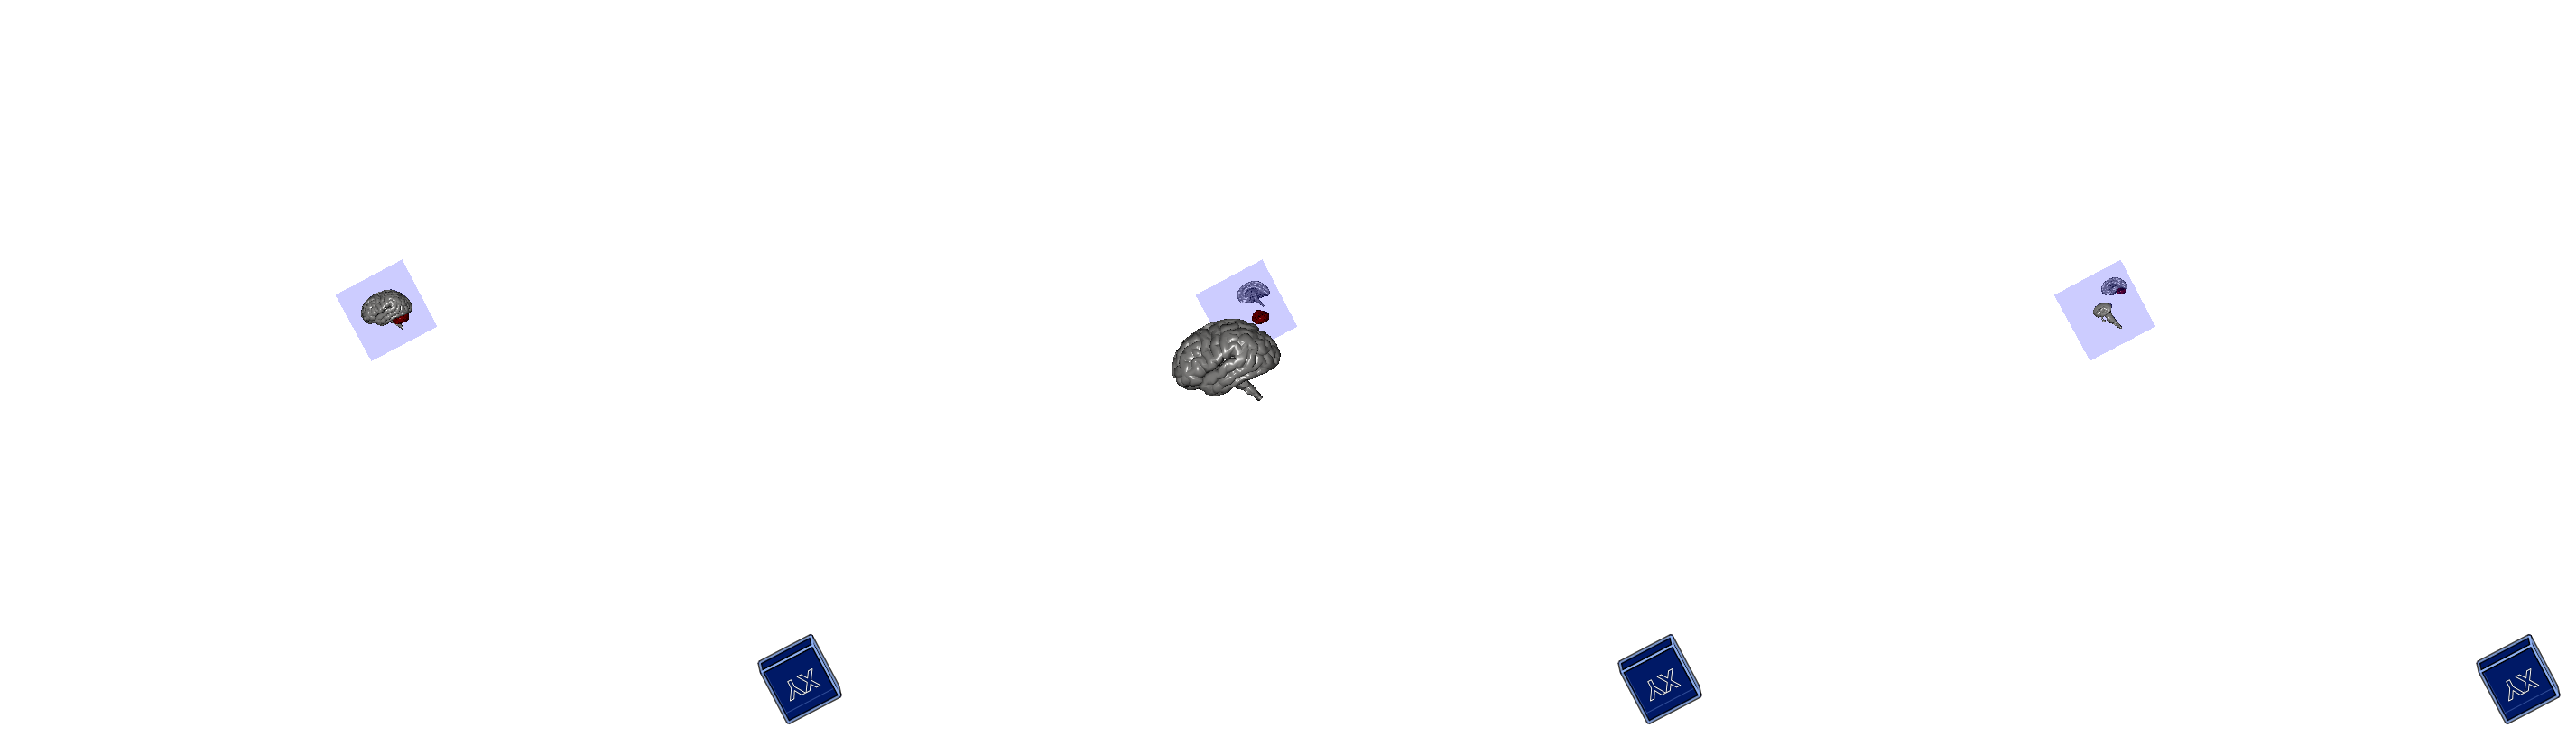
\includegraphics[width=0.9\textwidth]{chapters/figures/infinity}
	\caption{Different objects of interest from roghly the same viewpoint caus the offset to grow, placing the object out of view}
	\label{fig:infinity}
\end{figure}
To circumvent this problem I defined a maximum offset $o_{max}$ of the objects diameter which is the length of the distance between the minimum and maximum corners of the bounding box of the mesh. Since the mesh itself has no bounding box, the bounding box has to be accumulated by combining the bounding boxes of the groups of the mesh. This way the distance between the exploded parts can never exceed twice the diameter of the object.\\
To avoid parts of the object of interest now being occluded I used a simple ghosting technique: 
The front part, meaning the exploded part that is between the viewer and the split plane, is being rendered translucently if the distance becomes too large.
If the current offset $o_c$ exceeds $o_{max} \cdot 0.7$ the opacity $\alpha$ of the front part is linearly interpolated between $1.0$ at $o_c = o_{max} \cdot 0.7$ and $0.5$ at  $o_c = o_{max}$ using the formula
\begin{equation}
	\alpha = \frac{o_{max}-o_c}{o_{max} \cdot 0.3} \cdot 0.5 + 0.5
\end{equation}
This opacity factor $\alpha$ is then multiplied by $r$ so that the object stays solid while its not occluding anything and is most translucent if the whole object of interest is occluded completely.\\
To determine which part is the front part, I calculated the dot product of the viewing vector and the plane normal, using its sign to determine whether the part shifted in direction of the plane normal is the front part or not. This also determines in which order the parts are rendered, with the front part being the last, so that it can be translucently blended over the solid parts.\\
A problem that now appears is that backface culling is deactivated to so that the cutaway can be rendered correctly, resulting in the translucent objects' backfaces also visible, which causes the graphic to appear slightly confusing and aesthetically unpleasant. This can be avoided by allowing backface culling for a translucent object, if its offset vector doesn't point away from the camera. Because this may be the case if the camera is placed between the original and the translated switch plane, the dot product has to be calculated once more, now for the translated split plane.\\
\begin{figure}[tb]
	\centering
	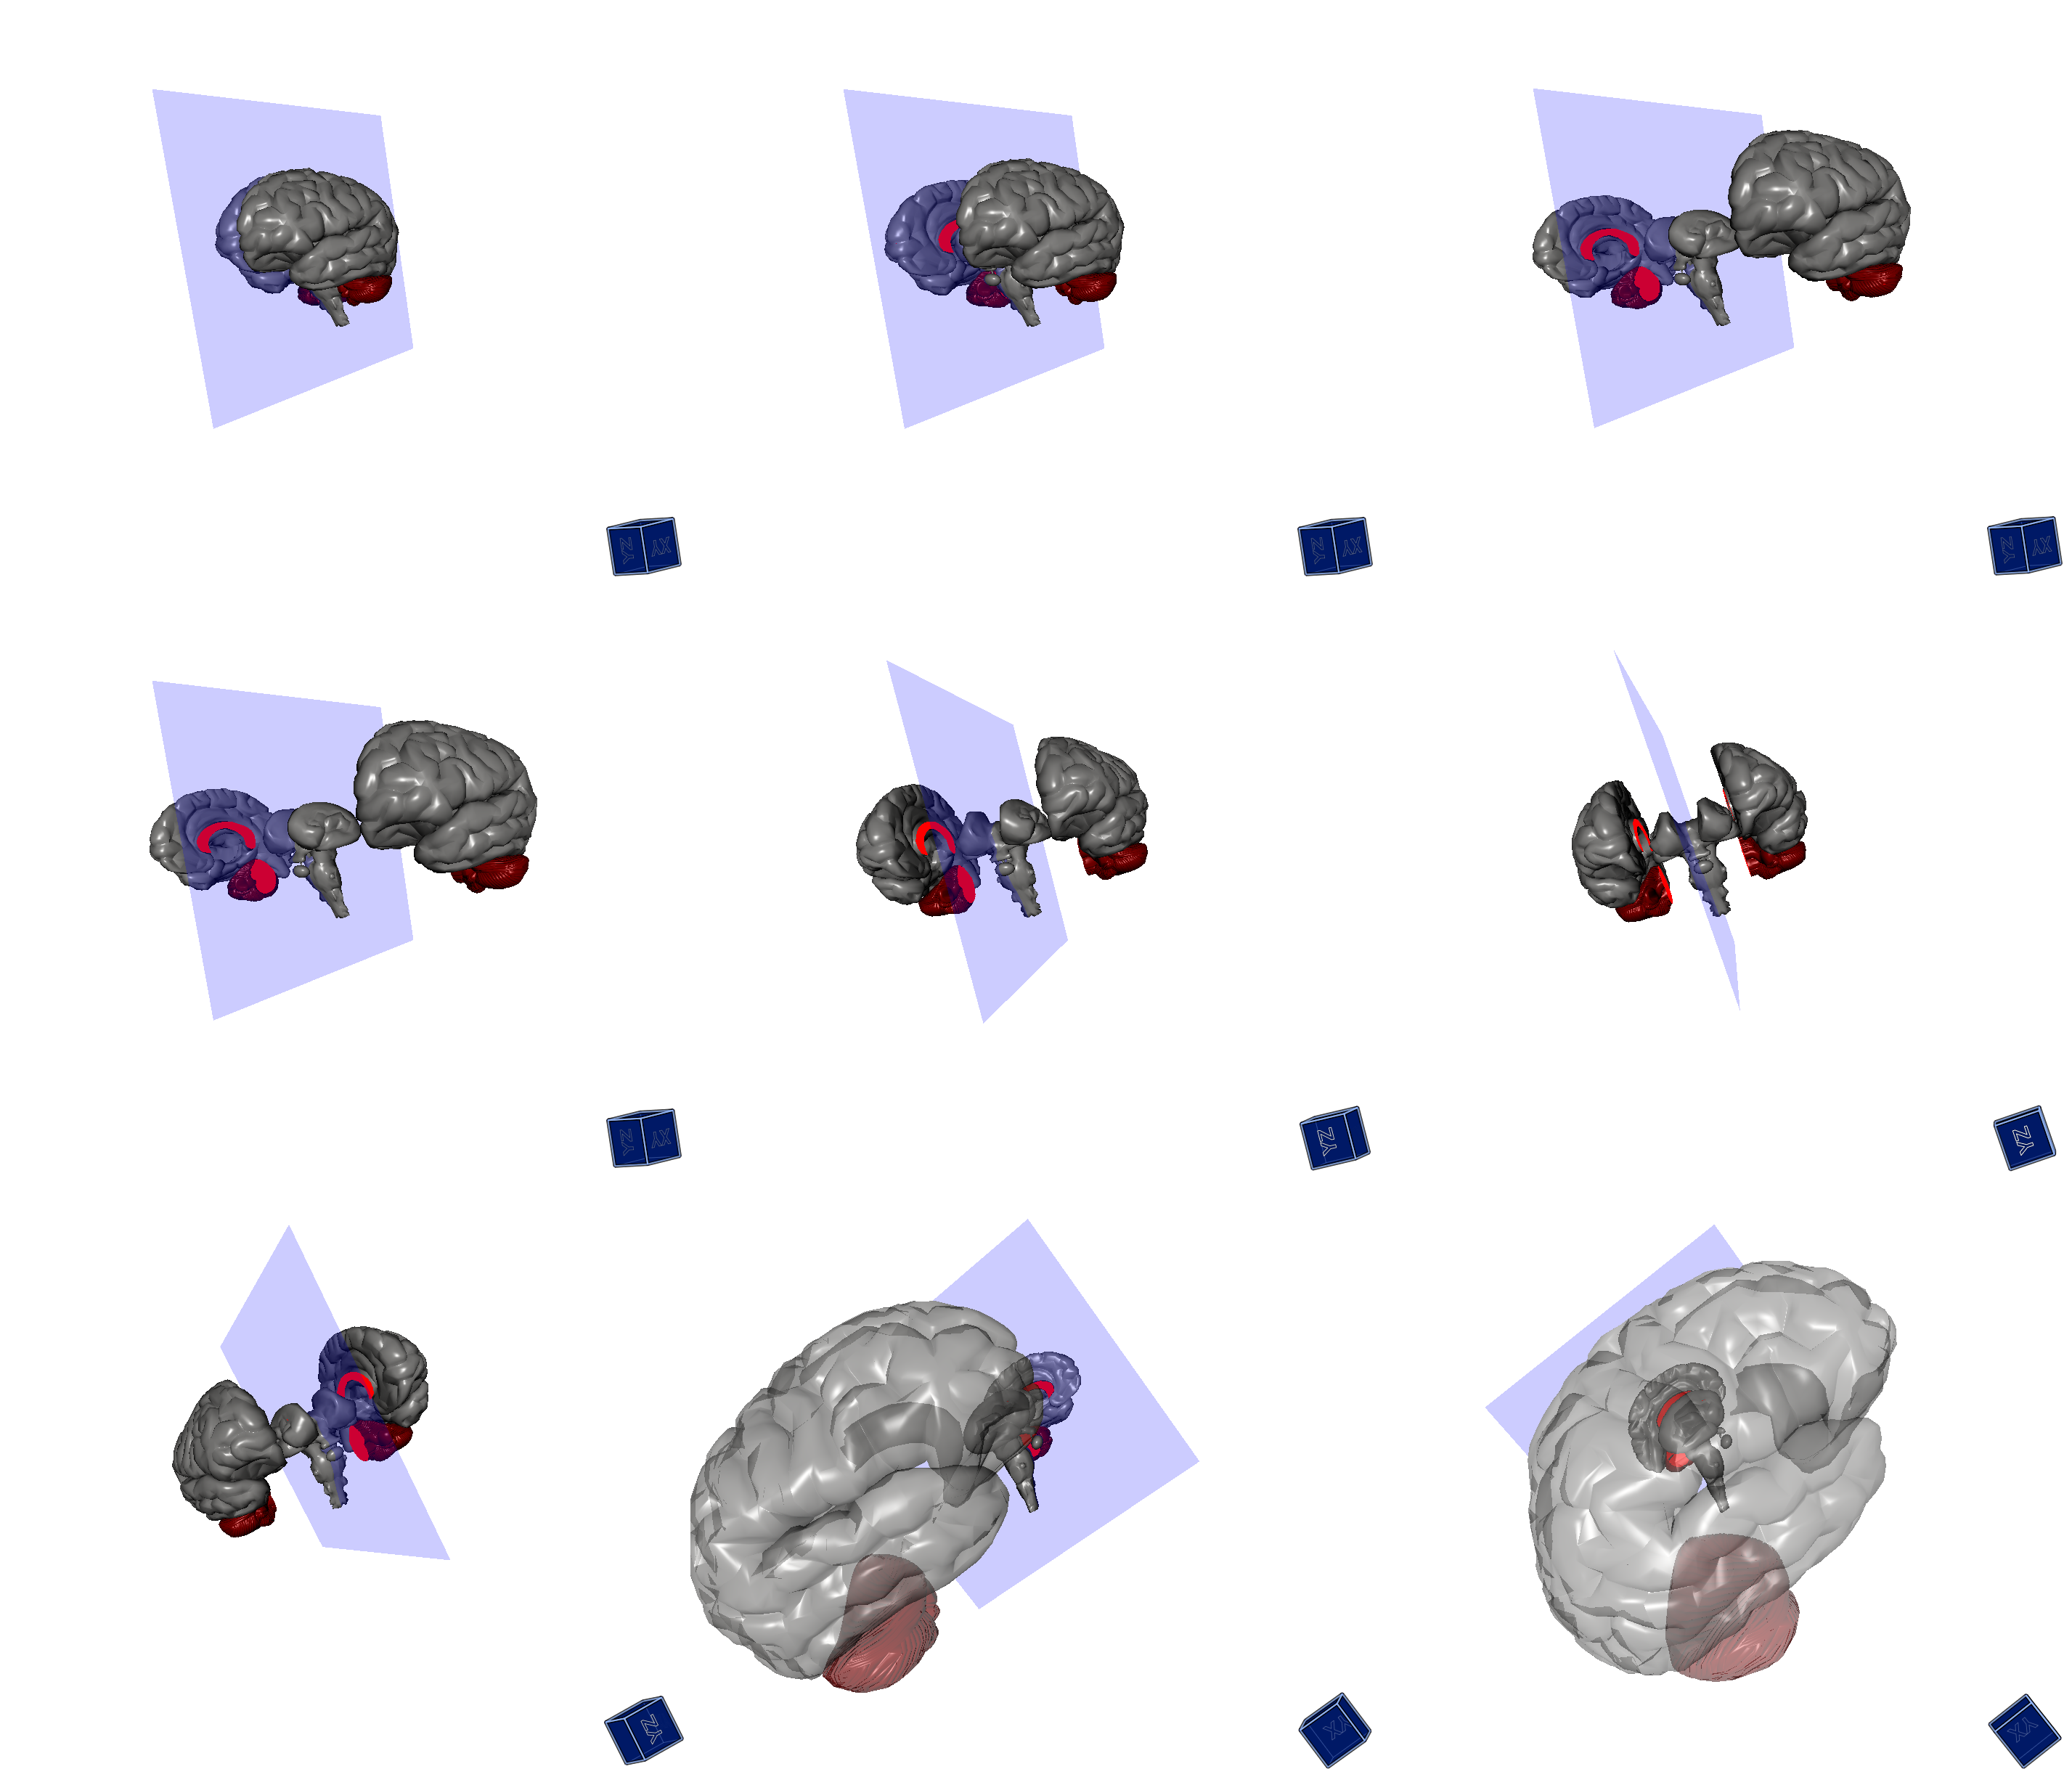
\includegraphics[width=0.9\textwidth]{chapters/figures/brainstem}
	\caption{Depiction of the animations and ghosting in the final version of the plugin}
	\label{fig:brainstem}
\end{figure}
\chapter{Conclusion}
In general I think that the combination of ghosting and exploded views in this form is not an ideal one, one of the main advantages of ghosting, that all parts of the object appear in their original location, is lost, but in comparison to the behavior the pure explosive view exhibits when viewed from angles close to the explosion direction it gives more information about the object of interest and it looks better than a solid part blocking it or disappearing from view.
\subsubsection{Future Work}
At the moment the explosive view is very simple, it would bew interesting to create something with multible axes more complex assemblies.

%%%%%%%%%%%%%%%%%%%%%%%%%%%%%%%%%%%%%%%%%
%\chapter{Bibliographic Issues}
%\label{ch:bibliographic}
%%%%%%%%%%%%%%%%%%%%%%%%%%%%%%%%%%%%%%%%%

%%\section{Literature Search}
%
%Information on online libraries and literature search, e.g., interesting magazines, journals, conferences, and organizations may be found at \url{http://www.big.tuwien.ac.at/teaching/info.html}.
%
%\section{BibTeX}
%
%BibTeX should be used for referencing.
%
%The \LaTeX source document of this pdf document provides you with different samples for references to journals~\cite{jour:B2BServices}, conference papers~\cite{proc:TheWebMLApproachi}, books~\cite{book:umlatwork}, book chapters~\cite{incoll:ErhardKonrad1992}, electronic standards~\cite{man:BPEL}, dissertations~\cite{phdthesis:manuelWimmer}, masters' theses~\cite{mast:AUMLProfile}, and web sites~\cite{misc:BIGWebsite}. The respective BibTeX entries may be found in the file \texttt{references.bib}. For administration of the BibTeX references we recommend \url{http://www.citeulike.org} or JabRef for offline administration, respectively.
bruckner-2006-EVV\cite{proc:bruckner-2006-EVV}\\
ruiz \cite{proc:ruiz-2008-SEV} \\
Li:2008\cite{proc:Li:2008:AGI} \\
og/AgrawalaPHHKHT\cite{journals/tog/AgrawalaPHHKHT03}\\
roc:conf/si3d/NiederauerHAH03\cite{proc:conf/si3d/NiederauerHAH03}\\
Viola-05-Smart\cite{Viola-05-Smart}\\
journals/cacm/MitraYYLA13\cite{journals/cacm/MitraYYLA13}\\
Ward:2010:IDV:1893097\cite{Ward:2010:IDV:1893097}\\


%%%%%%%%%%%%%%%%%%%%%%%%%%%%%%%%%%%%%%%%%
%%% BACKMATTER %%%%%%%%%%%%%%%%%%%%%%%%%%
%%%%%%%%%%%%%%%%%%%%%%%%%%%%%%%%%%%%%%%%%
\appendix

\bibliographystyle{plain}
\bibliography{chapters/references}

\end{document}
